% Options for packages loaded elsewhere
\PassOptionsToPackage{unicode}{hyperref}
\PassOptionsToPackage{hyphens}{url}
%
\documentclass[
]{book}
\usepackage{lmodern}
\usepackage{amssymb,amsmath}
\usepackage{ifxetex,ifluatex}
\ifnum 0\ifxetex 1\fi\ifluatex 1\fi=0 % if pdftex
  \usepackage[T1]{fontenc}
  \usepackage[utf8]{inputenc}
  \usepackage{textcomp} % provide euro and other symbols
\else % if luatex or xetex
  \usepackage{unicode-math}
  \defaultfontfeatures{Scale=MatchLowercase}
  \defaultfontfeatures[\rmfamily]{Ligatures=TeX,Scale=1}
\fi
% Use upquote if available, for straight quotes in verbatim environments
\IfFileExists{upquote.sty}{\usepackage{upquote}}{}
\IfFileExists{microtype.sty}{% use microtype if available
  \usepackage[]{microtype}
  \UseMicrotypeSet[protrusion]{basicmath} % disable protrusion for tt fonts
}{}
\makeatletter
\@ifundefined{KOMAClassName}{% if non-KOMA class
  \IfFileExists{parskip.sty}{%
    \usepackage{parskip}
  }{% else
    \setlength{\parindent}{0pt}
    \setlength{\parskip}{6pt plus 2pt minus 1pt}}
}{% if KOMA class
  \KOMAoptions{parskip=half}}
\makeatother
\usepackage{xcolor}
\IfFileExists{xurl.sty}{\usepackage{xurl}}{} % add URL line breaks if available
\IfFileExists{bookmark.sty}{\usepackage{bookmark}}{\usepackage{hyperref}}
\hypersetup{
  pdftitle={Bitácora},
  pdfauthor={Francisco Murphy Pérez},
  hidelinks,
  pdfcreator={LaTeX via pandoc}}
\urlstyle{same} % disable monospaced font for URLs
\usepackage{color}
\usepackage{fancyvrb}
\newcommand{\VerbBar}{|}
\newcommand{\VERB}{\Verb[commandchars=\\\{\}]}
\DefineVerbatimEnvironment{Highlighting}{Verbatim}{commandchars=\\\{\}}
% Add ',fontsize=\small' for more characters per line
\usepackage{framed}
\definecolor{shadecolor}{RGB}{248,248,248}
\newenvironment{Shaded}{\begin{snugshade}}{\end{snugshade}}
\newcommand{\AlertTok}[1]{\textcolor[rgb]{0.94,0.16,0.16}{#1}}
\newcommand{\AnnotationTok}[1]{\textcolor[rgb]{0.56,0.35,0.01}{\textbf{\textit{#1}}}}
\newcommand{\AttributeTok}[1]{\textcolor[rgb]{0.77,0.63,0.00}{#1}}
\newcommand{\BaseNTok}[1]{\textcolor[rgb]{0.00,0.00,0.81}{#1}}
\newcommand{\BuiltInTok}[1]{#1}
\newcommand{\CharTok}[1]{\textcolor[rgb]{0.31,0.60,0.02}{#1}}
\newcommand{\CommentTok}[1]{\textcolor[rgb]{0.56,0.35,0.01}{\textit{#1}}}
\newcommand{\CommentVarTok}[1]{\textcolor[rgb]{0.56,0.35,0.01}{\textbf{\textit{#1}}}}
\newcommand{\ConstantTok}[1]{\textcolor[rgb]{0.00,0.00,0.00}{#1}}
\newcommand{\ControlFlowTok}[1]{\textcolor[rgb]{0.13,0.29,0.53}{\textbf{#1}}}
\newcommand{\DataTypeTok}[1]{\textcolor[rgb]{0.13,0.29,0.53}{#1}}
\newcommand{\DecValTok}[1]{\textcolor[rgb]{0.00,0.00,0.81}{#1}}
\newcommand{\DocumentationTok}[1]{\textcolor[rgb]{0.56,0.35,0.01}{\textbf{\textit{#1}}}}
\newcommand{\ErrorTok}[1]{\textcolor[rgb]{0.64,0.00,0.00}{\textbf{#1}}}
\newcommand{\ExtensionTok}[1]{#1}
\newcommand{\FloatTok}[1]{\textcolor[rgb]{0.00,0.00,0.81}{#1}}
\newcommand{\FunctionTok}[1]{\textcolor[rgb]{0.00,0.00,0.00}{#1}}
\newcommand{\ImportTok}[1]{#1}
\newcommand{\InformationTok}[1]{\textcolor[rgb]{0.56,0.35,0.01}{\textbf{\textit{#1}}}}
\newcommand{\KeywordTok}[1]{\textcolor[rgb]{0.13,0.29,0.53}{\textbf{#1}}}
\newcommand{\NormalTok}[1]{#1}
\newcommand{\OperatorTok}[1]{\textcolor[rgb]{0.81,0.36,0.00}{\textbf{#1}}}
\newcommand{\OtherTok}[1]{\textcolor[rgb]{0.56,0.35,0.01}{#1}}
\newcommand{\PreprocessorTok}[1]{\textcolor[rgb]{0.56,0.35,0.01}{\textit{#1}}}
\newcommand{\RegionMarkerTok}[1]{#1}
\newcommand{\SpecialCharTok}[1]{\textcolor[rgb]{0.00,0.00,0.00}{#1}}
\newcommand{\SpecialStringTok}[1]{\textcolor[rgb]{0.31,0.60,0.02}{#1}}
\newcommand{\StringTok}[1]{\textcolor[rgb]{0.31,0.60,0.02}{#1}}
\newcommand{\VariableTok}[1]{\textcolor[rgb]{0.00,0.00,0.00}{#1}}
\newcommand{\VerbatimStringTok}[1]{\textcolor[rgb]{0.31,0.60,0.02}{#1}}
\newcommand{\WarningTok}[1]{\textcolor[rgb]{0.56,0.35,0.01}{\textbf{\textit{#1}}}}
\usepackage{longtable,booktabs}
% Correct order of tables after \paragraph or \subparagraph
\usepackage{etoolbox}
\makeatletter
\patchcmd\longtable{\par}{\if@noskipsec\mbox{}\fi\par}{}{}
\makeatother
% Allow footnotes in longtable head/foot
\IfFileExists{footnotehyper.sty}{\usepackage{footnotehyper}}{\usepackage{footnote}}
\makesavenoteenv{longtable}
\usepackage{graphicx}
\makeatletter
\def\maxwidth{\ifdim\Gin@nat@width>\linewidth\linewidth\else\Gin@nat@width\fi}
\def\maxheight{\ifdim\Gin@nat@height>\textheight\textheight\else\Gin@nat@height\fi}
\makeatother
% Scale images if necessary, so that they will not overflow the page
% margins by default, and it is still possible to overwrite the defaults
% using explicit options in \includegraphics[width, height, ...]{}
\setkeys{Gin}{width=\maxwidth,height=\maxheight,keepaspectratio}
% Set default figure placement to htbp
\makeatletter
\def\fps@figure{htbp}
\makeatother
\setlength{\emergencystretch}{3em} % prevent overfull lines
\providecommand{\tightlist}{%
  \setlength{\itemsep}{0pt}\setlength{\parskip}{0pt}}
\setcounter{secnumdepth}{5}
\usepackage{booktabs}
\usepackage{booktabs}
\usepackage{longtable}
\usepackage{array}
\usepackage{multirow}
\usepackage{wrapfig}
\usepackage{float}
\usepackage{colortbl}
\usepackage{pdflscape}
\usepackage{tabu}
\usepackage{threeparttable}
\usepackage{threeparttablex}
\usepackage[normalem]{ulem}
\usepackage{makecell}
\usepackage{xcolor}
\usepackage[]{natbib}
\bibliographystyle{apalike}

\title{Bitácora}
\author{Francisco Murphy Pérez}
\date{2020-06-27}

\begin{document}
\maketitle

{
\setcounter{tocdepth}{1}
\tableofcontents
}
\hypertarget{resumen-del-proyecto}{%
\chapter{Resumen del proyecto}\label{resumen-del-proyecto}}

Bitácora del proyecto de doctorado de Francisco Murphy Pérez.

En resumen, el proyecto de doctorado consiste en analizar el efecto que tiene el pH en el daño por radiación en cristales de proteína. Para ello se plantea cristalizar algunas proteínas con la misma condición de cristalización pero diferente pH.

La primer parte trata de obtener una lista de proteínas que cumplan los requisitos \emph{adecuados} para llevar a cabo dicho proyecto.

La segunda parte será la reproducción de las condiciones de cristalización de las proteínas adecuadas.

En la tercera parte del proyecto se realizará un análisis del daño por radiación en los cristales obtenidos.

\hypertarget{contacto}{%
\section{Contacto}\label{contacto}}

Me puedes contactar por correo electrónico en \href{mailto:murpholinox@gmail.com}{gmail} o \href{mailto:murphy@ibt.unam.mx}{ibt}.

\hypertarget{dependencias}{%
\chapter{Dependencias}\label{dependencias}}

Se listan las dependencias usadas.

\hypertarget{ejecuta-cuxf3digo}{%
\section{Ejecuta código}\label{ejecuta-cuxf3digo}}

\begin{Shaded}
\begin{Highlighting}[]
\CommentTok{\# knitr::opts\_chunk$set(eval = FALSE)}
\end{Highlighting}
\end{Shaded}

\hypertarget{configuraciuxf3n}{%
\section{Configuración}\label{configuraciuxf3n}}

Se cargan las librerías necesarias de \texttt{R}.

\begin{Shaded}
\begin{Highlighting}[]
\KeywordTok{library}\NormalTok{(dplyr)}
\KeywordTok{library}\NormalTok{(ggplot2)}
\KeywordTok{library}\NormalTok{(readr)}
\KeywordTok{library}\NormalTok{(knitr)}
\KeywordTok{library}\NormalTok{(kableExtra)}
\KeywordTok{library}\NormalTok{(stringdist)}
\KeywordTok{library}\NormalTok{(svglite)}
\end{Highlighting}
\end{Shaded}

\hypertarget{sesiuxf3n}{%
\section{Sesión}\label{sesiuxf3n}}

Imprime información de la sesión activa de \texttt{R}.

\begin{Shaded}
\begin{Highlighting}[]
\KeywordTok{sessionInfo}\NormalTok{()}
\end{Highlighting}
\end{Shaded}

\begin{verbatim}
## R version 3.6.3 (2020-02-29)
## Platform: x86_64-redhat-linux-gnu (64-bit)
## Running under: Fedora 32 (Workstation Edition)
## 
## Matrix products: default
## BLAS/LAPACK: /usr/lib64/libopenblas-r0.3.9.so
## 
## locale:
##  [1] LC_CTYPE=en_US.UTF-8       LC_NUMERIC=C              
##  [3] LC_TIME=en_US.UTF-8        LC_COLLATE=en_US.UTF-8    
##  [5] LC_MONETARY=en_US.UTF-8    LC_MESSAGES=en_US.UTF-8   
##  [7] LC_PAPER=en_US.UTF-8       LC_NAME=C                 
##  [9] LC_ADDRESS=C               LC_TELEPHONE=C            
## [11] LC_MEASUREMENT=en_US.UTF-8 LC_IDENTIFICATION=C       
## 
## attached base packages:
## [1] stats     graphics  grDevices datasets  utils     methods   base     
## 
## other attached packages:
## [1] svglite_1.2.3      stringdist_0.9.5.5 kableExtra_1.1.0   knitr_1.28        
## [5] readr_1.3.1        ggplot2_3.3.1      dplyr_1.0.0       
## 
## loaded via a namespace (and not attached):
##  [1] Rcpp_1.0.4.6      pillar_1.4.4      compiler_3.6.3    tools_3.6.3      
##  [5] digest_0.6.25     viridisLite_0.3.0 evaluate_0.14     lifecycle_0.2.0  
##  [9] tibble_3.0.1      gtable_0.3.0      pkgconfig_2.0.3   rlang_0.4.6      
## [13] rstudioapi_0.11   parallel_3.6.3    yaml_2.2.1        xfun_0.14        
## [17] xml2_1.3.2        withr_2.2.0       stringr_1.4.0     httr_1.4.1       
## [21] systemfonts_0.2.3 gdtools_0.2.2     generics_0.0.2    vctrs_0.3.1      
## [25] hms_0.5.3         webshot_0.5.2     grid_3.6.3        tidyselect_1.1.0 
## [29] glue_1.4.1        R6_2.4.1          rmarkdown_2.2     bookdown_0.19    
## [33] purrr_0.3.4       magrittr_1.5      scales_1.1.1      ellipsis_0.3.1   
## [37] htmltools_0.4.0   rvest_0.3.5       colorspace_1.4-1  renv_0.10.0      
## [41] stringi_1.4.6     munsell_0.5.0     crayon_1.3.4
\end{verbatim}

\hypertarget{sistema-operativo}{%
\section{Sistema operativo}\label{sistema-operativo}}

Como se nota en la salida anterior, el sistema operativo usado es Fedora 32 (\url{https://getfedora.org/}) en su versión \emph{workstation}.

\begin{Shaded}
\begin{Highlighting}[]
\FunctionTok{uname}\NormalTok{ {-}r }\CommentTok{\# Imprime versión del núcleo de linux.}
\end{Highlighting}
\end{Shaded}

\begin{verbatim}
## 5.6.15-300.fc32.x86_64
\end{verbatim}

\hypertarget{mineruxeda-de-datos}{%
\section{Minería de datos}\label{mineruxeda-de-datos}}

La extracción de datos se realiza con \texttt{gemmi} (\url{https://github.com/project-gemmi/gemmi}). Cuya instalación depende a su vez de \texttt{git} y \texttt{cmake}.

\begin{Shaded}
\begin{Highlighting}[]
\FunctionTok{sudo}\NormalTok{ dnf {-}y install git cmake}
\BuiltInTok{cd}\KeywordTok{;} \FunctionTok{mkdir}\NormalTok{ Repos}\KeywordTok{;} \BuiltInTok{cd}\NormalTok{ Repos}
\FunctionTok{git}\NormalTok{ clone https://github.com/project{-}gemmi/gemmi.git}
\BuiltInTok{cd}\NormalTok{ gemmi}
\FunctionTok{cmake}\NormalTok{ .}
\FunctionTok{make}
\BuiltInTok{echo} \StringTok{"\# Gemmi"} \OperatorTok{\textgreater{}\textgreater{}}\NormalTok{ \textasciitilde{}/.bashrc}
\BuiltInTok{echo} \StringTok{"alias gemmi=\textquotesingle{}/home/murphy/Repos/gemmi/gemmi\textquotesingle{}"} \OperatorTok{\textgreater{}\textgreater{}}\NormalTok{ \textasciitilde{}/.bashrc}
\end{Highlighting}
\end{Shaded}

Y para la transformación y limpieza de datos se usa:

\begin{itemize}
\tightlist
\item
  \texttt{grep} (\url{https://www.gnu.org/software/grep/})
\item
  \texttt{awk} (\url{https://www.gnu.org/software/gawk/})
\item
  \texttt{sed} (\url{https://www.gnu.org/software/gawk/})
\item
  \texttt{R} (\url{https://www.r-project.org/})
\item
  \texttt{tidyverse} (\url{https://www.tidyverse.org/})
\item
  \texttt{bash} (\url{https://www.gnu.org/software/bash/})
\end{itemize}

La instalación de \texttt{R} conviene hacerla como lo describo en el siguiente enlace \url{https://murpholinox.github.io/installRwithouttexlivedependencies/}.

La instalación del \texttt{tidyverse} depende a su vez de la instalación de las siguientes librerías en el SO.

\begin{Shaded}
\begin{Highlighting}[]
\FunctionTok{sudo}\NormalTok{ dnf {-}y install openssl{-}devel libxml2{-}devel libcurl{-}devel}
\end{Highlighting}
\end{Shaded}

\hypertarget{bituxe1cora}{%
\subsection{Bitácora}\label{bituxe1cora}}

La reproducción correcta, desde la ejecución del código hasta la producción del archivo de salida, de esta bitácora depende de la instalación de varios programas:

\begin{itemize}
\tightlist
\item
  \texttt{rstudio} (\url{https://rstudio.com/})
\item
  \texttt{bookdown} (\url{https://github.com/rstudio/bookdown})
\item
  \texttt{rmarkdown} (\url{https://rmarkdown.rstudio.com/})
\item
  \texttt{renv} (\url{https://github.com/rstudio/renv})
\end{itemize}

\begin{Shaded}
\begin{Highlighting}[]
\CommentTok{\# renv::consent() \# Da permiso a renv.}
\CommentTok{\# renv::init() \# Inicia renv.}
\end{Highlighting}
\end{Shaded}

\begin{Shaded}
\begin{Highlighting}[]
\CommentTok{\# Ve las dependencias.}
\FunctionTok{cat}\NormalTok{ renv.lock}
\end{Highlighting}
\end{Shaded}

\hypertarget{extracciuxf3n-de-datos}{%
\chapter{Extracción de datos}\label{extracciuxf3n-de-datos}}

\hypertarget{muxe9todo-anterior}{%
\section{Método anterior}\label{muxe9todo-anterior}}

En un inicio la extracción de datos se realizó por medio de la interfaz de programación de aplicaciones (API, por sus siglas en inglés) del banco de datos de proteínas (PDB, también por sus siglas en inglés), basado en una `búsqueda avanzada' en formato \texttt{.xml}, como lo describo en el siguiente enlace \url{https://murpholinox.github.io/getdatafromthePDB/}.

\hypertarget{cambios}{%
\section{Cambios}\label{cambios}}

A finales del 2019, se implementó una nueva API en el sitio \emph{web} del PDB que no permitió seguir con el proceso anterior, al introducir ciertas restricciones. Por lo menos a esta fecha, 30 de mayo 2020, las restricciones continúan y son las siguientes:

\begin{enumerate}
\def\labelenumi{\arabic{enumi}.}
\tightlist
\item
  Después de una `búsqueda avanzada', no es posible descargar el archivo \texttt{.csv} de los resultados de la búsqueda con un número mayor a 2500 líneas.
\end{enumerate}

\begin{figure}
\centering
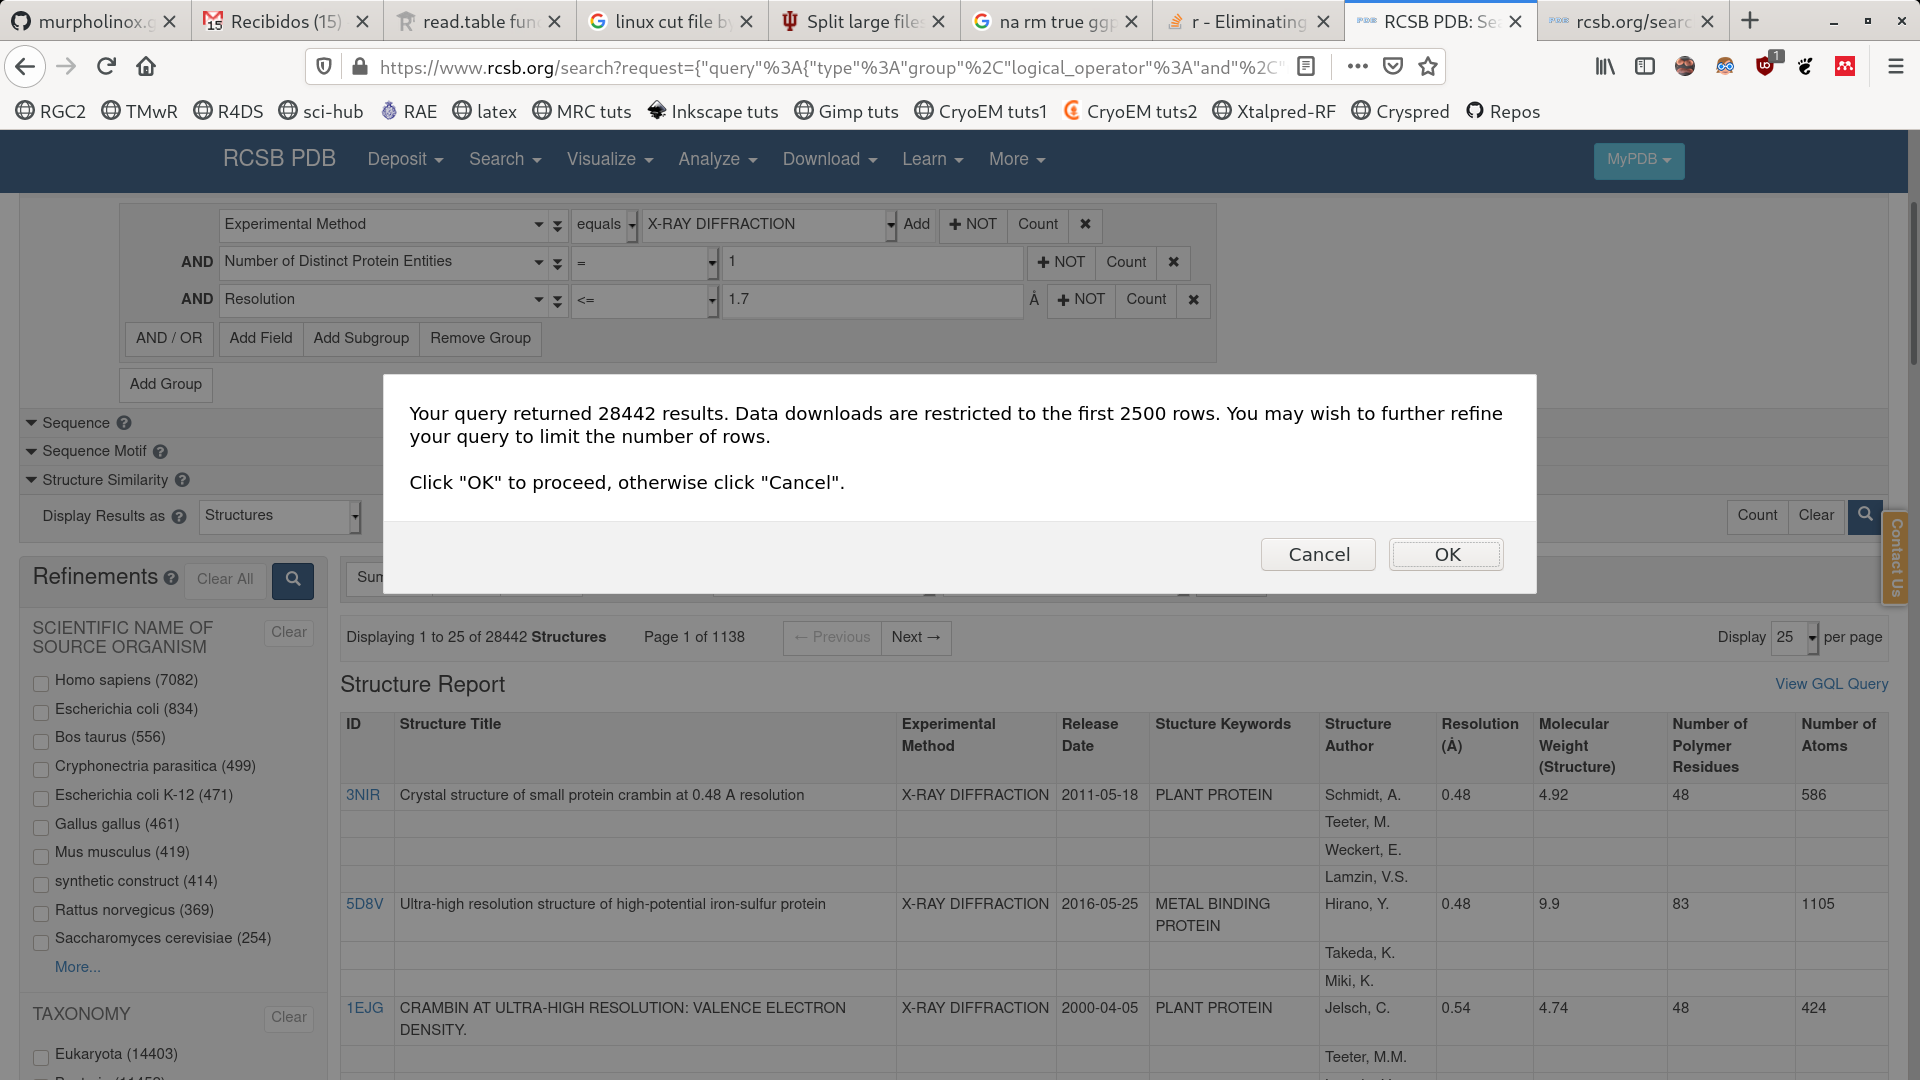
\includegraphics{/home/murphy/Repos/arrozconleche/img/2500rows.png}
\caption{Restricciones en el PDB}
\end{figure}

\begin{enumerate}
\def\labelenumi{\arabic{enumi}.}
\setcounter{enumi}{1}
\tightlist
\item
  Después de una `búsqueda avanzada', la opción de descargar un \texttt{.csv} personalizado, es decir, con la posibilidad de seleccionar las columnas de interés, no se encuentra disponible.
\end{enumerate}

\hypertarget{nuevo-muxe9todo}{%
\section{Nuevo método}\label{nuevo-muxe9todo}}

A causa de lo anterior se decidió emplear la información cruda del PDB, es decir, extraer la información directamente del cabezal de los archivos de las estructuras depositadas en el PDB.

\hypertarget{escoge-formato}{%
\subsection{Escoge formato}\label{escoge-formato}}

El PDB ofrece descargar sus archivos en tres formatos diferentes: \texttt{.xml}, \texttt{.pdb} y \texttt{.mmcif}. El segundo es el más fácil de leer y manipular; sin embargo, se decidió usar el tercer formato debido al siguiente párrafo:

\begin{quote}
Many of the errors have been fixed in the equivalent mmCIF files. Hence, if you are interested in the header information, it is a good idea to extract information from mmCIF files\ldots{}

De \url{https://biopython.readthedocs.io/en/latest/chapter_pdb.html}.
\end{quote}

\hypertarget{conoce-el-formato}{%
\subsection{Conoce el formato}\label{conoce-el-formato}}

El formato \texttt{.mmcif} se detalla en \url{http://mmcif.wwpdb.org/}. Existe una correspondencia entre las etiquetas del \texttt{.pdb} con las del \texttt{.mmcif}.

\begin{quote}
El formato \texttt{.mmcif}, tiene como fin reemplazar el formato \texttt{.pdb} (véase \url{http://mmcif.wwpdb.org/docs/faqs/pdbx-mmcif-faq-general.html}).
\end{quote}

\hypertarget{descarga-la-informaciuxf3n}{%
\subsection{Descarga la información}\label{descarga-la-informaciuxf3n}}

Para descargar todo las estructuras del PDB en formato \texttt{.mmcif}, se usa el siguiente comando:

\begin{Shaded}
\begin{Highlighting}[]
\BuiltInTok{cd}\NormalTok{ /run/media/murphy/lolita/doctorado }\CommentTok{\# Trabaja en el disco duro.}
\FunctionTok{rsync}\NormalTok{ {-}rlpt {-}v {-}z {-}{-}delete {-}{-}port=33444 rsync.rcsb.org::ftp\_data/structures/divided/mmCIF/ ./PDB }
\CommentTok{\# Tarda 725 minutos!}
\end{Highlighting}
\end{Shaded}

\begin{quote}
Instrucciones de \url{https://www.wwpdb.org/ftp/pdb-ftp-sites}.
\end{quote}

\hypertarget{organizaciuxf3n-de-la-informaciuxf3n}{%
\subsection{Organización de la información}\label{organizaciuxf3n-de-la-informaciuxf3n}}

Las estructuras están organizadas en diferentes subdirectorios, cuyo nombre está formado por el segundo y el tercer carácter del nombre del archivo \texttt{.mmcif}. Por ejemplo \texttt{1abc.mmcif} estará en el subdirectorio \texttt{ab/}. Para las pruebas se hace una copia de este directorio, sin los subdirectorios. Esto tiene dos fines: realizar un respaldo y manipular de una manera más sencilla los archivos.

\begin{Shaded}
\begin{Highlighting}[]
\BuiltInTok{cd}\NormalTok{ /run/media/murphy/lolita/doctorado}
\FunctionTok{mkdir}\NormalTok{ PDB\_backup}
\BuiltInTok{cd}\NormalTok{ PDB/}
\BuiltInTok{time}\NormalTok{ find . {-}name }\StringTok{\textquotesingle{}*.gz\textquotesingle{}}\NormalTok{ {-}exec cp }\DataTypeTok{\textbackslash{}\{\textbackslash{}\}}\NormalTok{ /run/media/murphy/lolita/doctorado/PDB\_backup/ }\DataTypeTok{\textbackslash{};} 
\CommentTok{\# Esto tarda 39m23.037s}
\CommentTok{\# Se confirma con:}
\CommentTok{\# cd ../PDB\_backup/}
\CommentTok{\# find {-}name "*.gz" | wc {-}l}
\CommentTok{\# 165650}
\end{Highlighting}
\end{Shaded}

Los archivos descargados están comprimidos en formato \texttt{gzip} (\url{https://www.gnu.org/software/gzip/}). No es necesario descomprimirlos.

\hypertarget{extracciuxf3n-de-datos-1}{%
\subsection{Extracción de datos}\label{extracciuxf3n-de-datos-1}}

La extracción de \texttt{gemmi} funciona de la siguiente manera:

\begin{Shaded}
\begin{Highlighting}[]
\CommentTok{\# Obtiene número de acceso.}
\CommentTok{\# time gemmi grep \_struct\_ref.pdbx\_db\_accession xrays/ \textgreater{} from\_xrays\_get\_ide}
\CommentTok{\# Esto tarda 83 minutos!}
\CommentTok{\# Obtiene número de entidades.}
\CommentTok{\# time gemmi grep \_entity\_poly.entity\_id xrays/ \textgreater{} from\_xrays\_get\_nde}
\CommentTok{\# Esto tarda 73 minutos!}
\CommentTok{\# Obtiene anteriores y tipo de entidad.}
\CommentTok{\# time gemmi grep \_struct\_ref.pdbx\_db\_accession {-}a \_entity\_poly.entity\_id {-}a \_entity\_poly.type xrays/ \textgreater{} from\_xrays\_get\_ide\_nde\_tde }
\CommentTok{\# Esto tarda 75 minutos!}
\CommentTok{\# Estos resultados no producen datos rectangulares, por la ausencia de un delimitador apropiado.}
\end{Highlighting}
\end{Shaded}

\hypertarget{separa-entradas-por-muxe9todo-experimental}{%
\subsubsection{Separa entradas por método experimental}\label{separa-entradas-por-muxe9todo-experimental}}

Del universo de archivos depositados en el PDB, obtenemos aquellas estructuras determinadas por cristalografía de rayos-X (CRX). Esto ayuda a reducir confusiones posteriores. Estas confusiones surgen porque \texttt{gemmi}, extrae etiquetas pero no conoce contextos. Esto puede resultar, dependiendo de las etiquetas, en una producción de un archivo de texto con un número de columnas variable por línea, es decir, datos en forma no rectangular.

\begin{quote}
Advertencia: La mayor parte del \texttt{tidyverse} trabaja con datos rectangulares, mismo número de columnas en todas las líneas, por lo que es esencial obtener datos de esta forma.
\end{quote}

\begin{Shaded}
\begin{Highlighting}[]
\BuiltInTok{cd}\NormalTok{ /run/media/murphy/lolita/doctorado/}
\FunctionTok{mkdir}\NormalTok{ extract}
\BuiltInTok{time}\NormalTok{ gemmi grep \_exptl.method PDB\_backup/ }\OperatorTok{\textgreater{}}\NormalTok{ ./extract/method.dat }
\CommentTok{\# Esto tarda 77m43.750s}
\CommentTok{\# Confirma con:}
\CommentTok{\# wc {-}l method.dat}
\CommentTok{\# 165820 }
\CommentTok{\# La diferencia es por los pdbs obtenidos vía múltiples métodos.}
\CommentTok{\# La siguiente línea nos da donde se da esta diferencia.}
\CommentTok{\# awk {-}F ":" \textquotesingle{}\{print $1\}\textquotesingle{} method.dat | uniq {-}c | awk \textquotesingle{}\{ if ($1!="1") print $0\}\textquotesingle{} \textgreater{} morethanonemethod.dat}
\BuiltInTok{cd}\NormalTok{ extract/}
\FunctionTok{grep}\NormalTok{ X{-}RAY method.dat }\KeywordTok{|} \FunctionTok{awk}\NormalTok{ {-}F : }\StringTok{\textquotesingle{}\{print $1\}\textquotesingle{}} \KeywordTok{|} \FunctionTok{tr} \StringTok{\textquotesingle{}[:upper:]\textquotesingle{}} \StringTok{\textquotesingle{}[:lower:]\textquotesingle{}} \OperatorTok{\textgreater{}}\NormalTok{ pdbs\_by\_xray.dat}
\FunctionTok{sed} \StringTok{\textquotesingle{}s/$/.cif.gz/\textquotesingle{}}\NormalTok{g pdbs\_by\_xray.dat }\OperatorTok{\textgreater{}}\NormalTok{ list\_pdbs\_by\_xray}
\CommentTok{\# Es interesante comparar el número de entradas por CRX contra el total:}
\CommentTok{\# wc {-}l pdbs\_by\_xray.dat}
\CommentTok{\# 147209 pdbs\_by\_xray.dat}
\CommentTok{\# El total era 165650, el cociente da = (147209/165650)*100=88.87}
\CommentTok{\# Es decir, 88.87 \% de las entradas en el PDB son por CRX.}
\FunctionTok{mkdir}\NormalTok{ xrays}
\BuiltInTok{time}\NormalTok{ cat list\_pdbs\_by\_xray }\KeywordTok{|} \KeywordTok{while} \BuiltInTok{read} \VariableTok{line}\NormalTok{;}
\KeywordTok{do} \FunctionTok{cp}\NormalTok{ /run/media/murphy/lolita/doctorado/PDB\_backup/}\VariableTok{$line}\NormalTok{ xrays/}\KeywordTok{;} \KeywordTok{done} 
\CommentTok{\# Esto tarda 51m51.134s!}
\end{Highlighting}
\end{Shaded}

\hypertarget{extrae-datos}{%
\subsubsection{Extrae datos}\label{extrae-datos}}

\begin{Shaded}
\begin{Highlighting}[]
\CommentTok{\# El primer delimitador usado fue \textless{}TAB\textgreater{} (\textbackslash{}t).}
\CommentTok{\# time gemmi grep {-}{-}delimiter=\textquotesingle{}\textbackslash{}t\textquotesingle{} \_entity\_poly.entity\_id {-}a \_entity\_poly.type {-}a \_struct\_ref.pdbx\_db\_accession {-}a \_entity.pdbx\_description {-}a \_exptl\_crystal\_grow.method {-}a \_exptl\_crystal\_grow.pH {-}a \_exptl\_crystal\_grow.pdbx\_details {-}a \_reflns.d\_resolution\_high {-}a \_reflns\_shell.d\_res\_high {-}a \_symmetry.space\_group\_name\_H{-}M {-}a \_citation.pdbx\_database\_id\_DOI xrays/ \textgreater{} todo}
\CommentTok{\# Esto tarda 45 minutos! }
\CommentTok{\# Estos resultados no producen datos rectangulares. }
\CommentTok{\# La causa es la presencia de \textless{}TAB\textgreater{} en la condición de cristalización.}
\CommentTok{\# La solución es usar un delimitador que no aparece en los archivos.}
\BuiltInTok{cd}\NormalTok{ /run/media/murphy/lolita/doctorado/extract}
\BuiltInTok{time}\NormalTok{ gemmi grep {-}{-}delimiter=}\StringTok{\textquotesingle{}¿\textquotesingle{}}\NormalTok{ \_entity\_poly.entity\_id {-}a \_entity\_poly.type {-}a \_struct\_ref.pdbx\_db\_accession {-}a \_entity.pdbx\_description {-}a \_exptl\_crystal\_grow.method {-}a \_exptl\_crystal\_grow.pH {-}a \_exptl\_crystal\_grow.pdbx\_details {-}a \_reflns.d\_resolution\_high {-}a \_reflns\_shell.d\_res\_high {-}a \_symmetry.space\_group\_name\_H{-}M {-}a \_citation.pdbx\_database\_id\_DOI xrays/ }\OperatorTok{\textgreater{}}\NormalTok{ information\_from\_xrays}
\CommentTok{\# Esto tarda 47m45.080s!}
\CommentTok{\# Por qué tarda menos cuando extrae más etiquetas?}
\CommentTok{\# Ni idea, pero es reproducible.}
\end{Highlighting}
\end{Shaded}

Importa los datos extraídos a \texttt{R} y los verifica realizando algunas gráficas interesantes.

\begin{Shaded}
\begin{Highlighting}[]
\KeywordTok{setwd}\NormalTok{(}\StringTok{"/run/media/murphy/lolita/doctorado/extract/"}\NormalTok{)}
\NormalTok{info \textless{}{-}}\StringTok{ }\KeywordTok{read\_delim}\NormalTok{(}\StringTok{"information\_from\_xrays"}\NormalTok{, }
    \StringTok{"¿"}\NormalTok{, }\DataTypeTok{escape\_double =} \OtherTok{FALSE}\NormalTok{, }\DataTypeTok{col\_names =} \OtherTok{FALSE}\NormalTok{, }
    \DataTypeTok{comment =} \StringTok{"*\textgreater{}"}\NormalTok{, }\DataTypeTok{trim\_ws =} \OtherTok{TRUE}\NormalTok{)}
\CommentTok{\# La configuración regional de mi sistema está en inglés.}
\CommentTok{\# \textasciigrave{}R\textasciigrave{} también por lo que no reconoce \textquotesingle{}¿\textquotesingle{}.}
\NormalTok{pdb\textless{}{-}info}\OperatorTok{$}\NormalTok{X1}
\NormalTok{nde\textless{}{-}stringr}\OperatorTok{::}\KeywordTok{str\_replace}\NormalTok{(info}\OperatorTok{$}\NormalTok{X2, }\StringTok{\textquotesingle{}�\textquotesingle{}}\NormalTok{, }\StringTok{\textquotesingle{}\textquotesingle{}}\NormalTok{)}
\NormalTok{tde\textless{}{-}stringr}\OperatorTok{::}\KeywordTok{str\_replace}\NormalTok{(info}\OperatorTok{$}\NormalTok{X3, }\StringTok{\textquotesingle{}�\textquotesingle{}}\NormalTok{, }\StringTok{\textquotesingle{}\textquotesingle{}}\NormalTok{)}
\NormalTok{ide\textless{}{-}stringr}\OperatorTok{::}\KeywordTok{str\_replace}\NormalTok{(info}\OperatorTok{$}\NormalTok{X4, }\StringTok{\textquotesingle{}�\textquotesingle{}}\NormalTok{, }\StringTok{\textquotesingle{}\textquotesingle{}}\NormalTok{)}
\NormalTok{nom\textless{}{-}stringr}\OperatorTok{::}\KeywordTok{str\_replace}\NormalTok{(info}\OperatorTok{$}\NormalTok{X5, }\StringTok{\textquotesingle{}�\textquotesingle{}}\NormalTok{, }\StringTok{\textquotesingle{}\textquotesingle{}}\NormalTok{)}
\NormalTok{tec\textless{}{-}stringr}\OperatorTok{::}\KeywordTok{str\_replace}\NormalTok{(info}\OperatorTok{$}\NormalTok{X6, }\StringTok{\textquotesingle{}�\textquotesingle{}}\NormalTok{, }\StringTok{\textquotesingle{}\textquotesingle{}}\NormalTok{)}
\NormalTok{peh\textless{}{-}stringr}\OperatorTok{::}\KeywordTok{str\_replace}\NormalTok{(info}\OperatorTok{$}\NormalTok{X7, }\StringTok{\textquotesingle{}�\textquotesingle{}}\NormalTok{, }\StringTok{\textquotesingle{}\textquotesingle{}}\NormalTok{)}
\NormalTok{con\textless{}{-}stringr}\OperatorTok{::}\KeywordTok{str\_replace}\NormalTok{(info}\OperatorTok{$}\NormalTok{X8, }\StringTok{\textquotesingle{}�\textquotesingle{}}\NormalTok{, }\StringTok{\textquotesingle{}\textquotesingle{}}\NormalTok{)}
\NormalTok{rs1\textless{}{-}stringr}\OperatorTok{::}\KeywordTok{str\_replace}\NormalTok{(info}\OperatorTok{$}\NormalTok{X9, }\StringTok{\textquotesingle{}�\textquotesingle{}}\NormalTok{, }\StringTok{\textquotesingle{}\textquotesingle{}}\NormalTok{)}
\NormalTok{rs2\textless{}{-}stringr}\OperatorTok{::}\KeywordTok{str\_replace}\NormalTok{(info}\OperatorTok{$}\NormalTok{X10, }\StringTok{\textquotesingle{}�\textquotesingle{}}\NormalTok{, }\StringTok{\textquotesingle{}\textquotesingle{}}\NormalTok{)}
\NormalTok{gpo\textless{}{-}stringr}\OperatorTok{::}\KeywordTok{str\_replace}\NormalTok{(info}\OperatorTok{$}\NormalTok{X11, }\StringTok{\textquotesingle{}�\textquotesingle{}}\NormalTok{, }\StringTok{\textquotesingle{}\textquotesingle{}}\NormalTok{)}
\NormalTok{doi\textless{}{-}stringr}\OperatorTok{::}\KeywordTok{str\_replace}\NormalTok{(info}\OperatorTok{$}\NormalTok{X12, }\StringTok{\textquotesingle{}�\textquotesingle{}}\NormalTok{, }\StringTok{\textquotesingle{}\textquotesingle{}}\NormalTok{)}
\NormalTok{datos\textless{}{-}}\KeywordTok{data.frame}\NormalTok{(pdb, nde, tde, ide, nom, tec, peh, con, rs1, rs2, gpo, doi)}
\KeywordTok{rm}\NormalTok{(pdb, nde, tde, ide, nom, tec, peh, con, rs1, rs2, gpo, doi)}
\CommentTok{\# Cuidado con el tipo de las columnas.}
\NormalTok{datos}\OperatorTok{$}\NormalTok{nde\textless{}{-}}\KeywordTok{as.numeric}\NormalTok{(}\KeywordTok{as.character}\NormalTok{((datos}\OperatorTok{$}\NormalTok{nde)))}
\NormalTok{datos}\OperatorTok{$}\NormalTok{peh\textless{}{-}}\KeywordTok{as.numeric}\NormalTok{(}\KeywordTok{as.character}\NormalTok{((datos}\OperatorTok{$}\NormalTok{peh)))}
\NormalTok{datos}\OperatorTok{$}\NormalTok{rs1\textless{}{-}}\KeywordTok{as.numeric}\NormalTok{(}\KeywordTok{as.character}\NormalTok{((datos}\OperatorTok{$}\NormalTok{rs1)))}
\NormalTok{datos}\OperatorTok{$}\NormalTok{rs2\textless{}{-}}\KeywordTok{as.numeric}\NormalTok{(}\KeywordTok{as.character}\NormalTok{((datos}\OperatorTok{$}\NormalTok{rs2)))}
\CommentTok{\# Verificamos los datos al graficar algunas variables interesantes:}
\KeywordTok{theme\_set}\NormalTok{(}\KeywordTok{theme\_bw}\NormalTok{())}
\CommentTok{\# Histograma del pH.}
\KeywordTok{ggplot}\NormalTok{(}\DataTypeTok{data =}\NormalTok{ datos, }\KeywordTok{aes}\NormalTok{(}\DataTypeTok{x=}\NormalTok{peh)) }\OperatorTok{+}\StringTok{ }\KeywordTok{geom\_histogram}\NormalTok{(}\DataTypeTok{binwidth =} \FloatTok{0.5}\NormalTok{) }\OperatorTok{+}\StringTok{ }\KeywordTok{labs}\NormalTok{(}\DataTypeTok{x=}\StringTok{"pH"}\NormalTok{, }\DataTypeTok{y=}\StringTok{"Frecuencia"}\NormalTok{) }\OperatorTok{+}\StringTok{ }\KeywordTok{xlim}\NormalTok{(}\DecValTok{1}\NormalTok{, }\DecValTok{11}\NormalTok{)}
\end{Highlighting}
\end{Shaded}

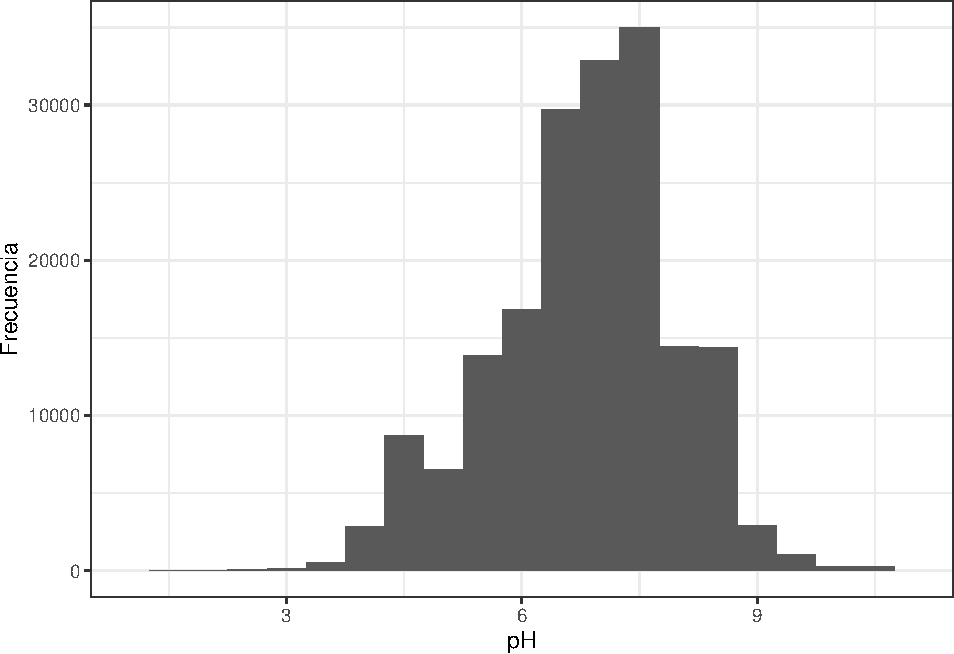
\includegraphics{arrozconleche_files/figure-latex/unnamed-chunk-14-1.pdf}

\begin{Shaded}
\begin{Highlighting}[]
\KeywordTok{ggsave}\NormalTok{(}\StringTok{"histograma\_todo\_xrays\_ph.png"}\NormalTok{, }\DataTypeTok{width =} \DecValTok{20}\NormalTok{, }\DataTypeTok{units =} \StringTok{"cm"}\NormalTok{)}
\KeywordTok{ggsave}\NormalTok{(}\StringTok{"histograma\_todo\_xrays\_ph.svg"}\NormalTok{, }\DataTypeTok{width =} \DecValTok{20}\NormalTok{, }\DataTypeTok{units =} \StringTok{"cm"}\NormalTok{)}
\CommentTok{\# Histograma de la resolución.}
\KeywordTok{ggplot}\NormalTok{(}\DataTypeTok{data =}\NormalTok{ datos, }\KeywordTok{aes}\NormalTok{(}\DataTypeTok{x=}\NormalTok{rs1)) }\OperatorTok{+}\StringTok{ }\KeywordTok{geom\_histogram}\NormalTok{(}\DataTypeTok{binwidth =} \FloatTok{0.1}\NormalTok{) }\OperatorTok{+}\StringTok{ }\KeywordTok{labs}\NormalTok{(}\DataTypeTok{x=}\StringTok{"Resolución (Å)"}\NormalTok{, }\DataTypeTok{y=}\StringTok{"Frecuencia"}\NormalTok{)}
\end{Highlighting}
\end{Shaded}

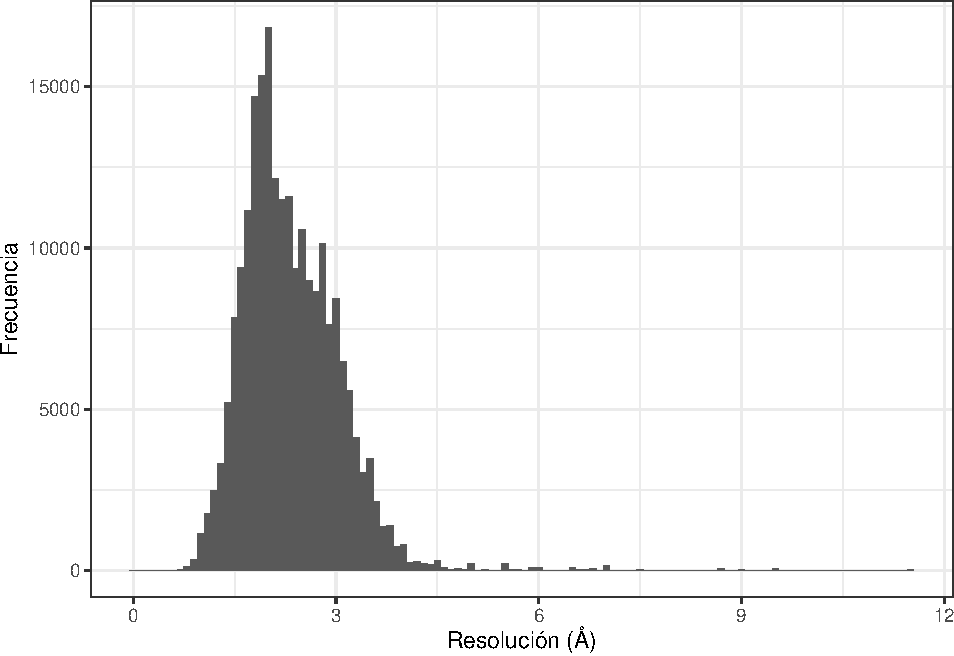
\includegraphics{arrozconleche_files/figure-latex/unnamed-chunk-14-2.pdf}

\begin{Shaded}
\begin{Highlighting}[]
\KeywordTok{ggsave}\NormalTok{(}\StringTok{"histograma\_todo\_xrays\_res.png"}\NormalTok{, }\DataTypeTok{width =} \DecValTok{20}\NormalTok{, }\DataTypeTok{units =} \StringTok{"cm"}\NormalTok{)}
\KeywordTok{ggsave}\NormalTok{(}\StringTok{"histograma\_todo\_xrays\_res.svg"}\NormalTok{, }\DataTypeTok{width =} \DecValTok{20}\NormalTok{, }\DataTypeTok{units =} \StringTok{"cm"}\NormalTok{)}
\CommentTok{\# Histograma del número de entidades.}
\KeywordTok{ggplot}\NormalTok{(}\DataTypeTok{data =}\NormalTok{ datos, }\KeywordTok{aes}\NormalTok{(}\DataTypeTok{x=}\NormalTok{nde)) }\OperatorTok{+}\StringTok{ }\KeywordTok{geom\_histogram}\NormalTok{(}\DataTypeTok{binwidth =} \DecValTok{1}\NormalTok{) }\OperatorTok{+}\StringTok{ }\KeywordTok{labs}\NormalTok{(}\DataTypeTok{x=}\StringTok{"Número de entidades"}\NormalTok{, }\DataTypeTok{y=}\StringTok{"Frecuencia"}\NormalTok{)}
\end{Highlighting}
\end{Shaded}

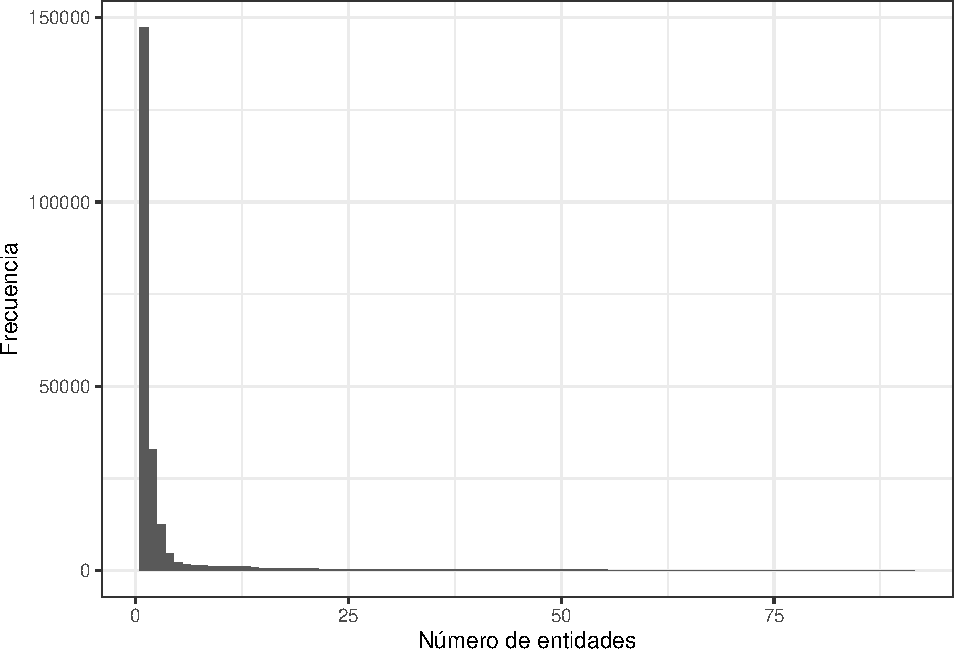
\includegraphics{arrozconleche_files/figure-latex/unnamed-chunk-14-3.pdf}

\begin{Shaded}
\begin{Highlighting}[]
\KeywordTok{ggsave}\NormalTok{(}\StringTok{"histograma\_todo\_xrays\_nde.png"}\NormalTok{, }\DataTypeTok{width =} \DecValTok{20}\NormalTok{, }\DataTypeTok{units =} \StringTok{"cm"}\NormalTok{)}
\KeywordTok{ggsave}\NormalTok{(}\StringTok{"histograma\_todo\_xrays\_nde.svg"}\NormalTok{, }\DataTypeTok{width =} \DecValTok{20}\NormalTok{, }\DataTypeTok{units =} \StringTok{"cm"}\NormalTok{)}
\CommentTok{\# Determina cuántos tipos de grupos espaciales y de entidades.}
\NormalTok{df1\textless{}{-}datos }\OperatorTok{\%\textgreater{}\%}
\StringTok{  }\KeywordTok{add\_count}\NormalTok{(gpo, }\DataTypeTok{name =} \StringTok{"cta\_gpo"}\NormalTok{)}
\NormalTok{df2\textless{}{-}df1 }\OperatorTok{\%\textgreater{}\%}
\StringTok{  }\KeywordTok{add\_count}\NormalTok{(tde, }\DataTypeTok{name =} \StringTok{"cta\_tde"}\NormalTok{)}
\NormalTok{tab\_gpo\textless{}{-}datos }\OperatorTok{\%\textgreater{}\%}
\StringTok{  }\KeywordTok{count}\NormalTok{(gpo, }\DataTypeTok{name =} \StringTok{"cta\_gpo"}\NormalTok{) }\OperatorTok{\%\textgreater{}\%}
\StringTok{  }\KeywordTok{arrange}\NormalTok{(}\KeywordTok{desc}\NormalTok{(cta\_gpo))}
\NormalTok{tab\_tde\textless{}{-}datos }\OperatorTok{\%\textgreater{}\%}
\StringTok{  }\KeywordTok{count}\NormalTok{(tde, }\DataTypeTok{name =} \StringTok{"cta\_tde"}\NormalTok{) }\OperatorTok{\%\textgreater{}\%}
\StringTok{  }\KeywordTok{arrange}\NormalTok{(}\KeywordTok{desc}\NormalTok{(cta\_tde))}
\CommentTok{\# Gráfico de barras de los grupos espaciales.}
\KeywordTok{ggplot}\NormalTok{(}\DataTypeTok{data =}\NormalTok{ df1, }\KeywordTok{aes}\NormalTok{(}\DataTypeTok{x=}\KeywordTok{reorder}\NormalTok{(gpo, cta\_gpo))) }\OperatorTok{+}\StringTok{ }\KeywordTok{geom\_bar}\NormalTok{() }\OperatorTok{+}\StringTok{ }\KeywordTok{labs}\NormalTok{(}\DataTypeTok{x=}\StringTok{"Grupo espacial"}\NormalTok{, }\DataTypeTok{y=}\StringTok{"Frecuencia"}\NormalTok{) }\OperatorTok{+}\StringTok{ }\KeywordTok{theme}\NormalTok{(}\DataTypeTok{axis.text.x =} \KeywordTok{element\_text}\NormalTok{(}\DataTypeTok{angle =} \DecValTok{90}\NormalTok{))}
\end{Highlighting}
\end{Shaded}

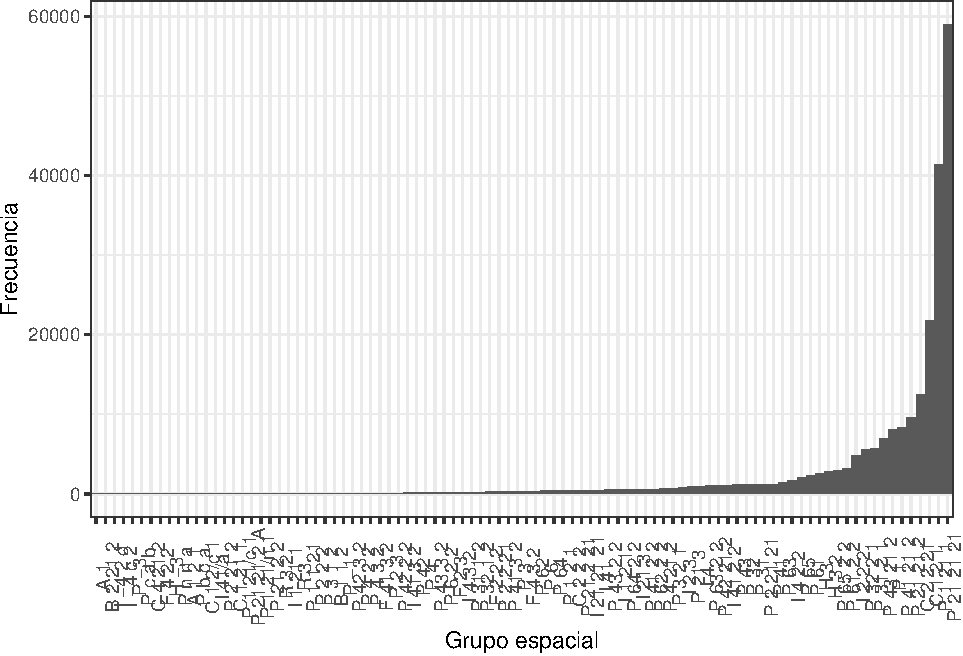
\includegraphics{arrozconleche_files/figure-latex/unnamed-chunk-14-4.pdf}

\begin{Shaded}
\begin{Highlighting}[]
\KeywordTok{ggsave}\NormalTok{(}\StringTok{"barras\_todo\_xrays\_gpo.png"}\NormalTok{, }\DataTypeTok{width =} \DecValTok{20}\NormalTok{, }\DataTypeTok{units =} \StringTok{"cm"}\NormalTok{)}
\KeywordTok{ggsave}\NormalTok{(}\StringTok{"barras\_todo\_xrays\_gpo.svg"}\NormalTok{, }\DataTypeTok{width =} \DecValTok{20}\NormalTok{, }\DataTypeTok{units =} \StringTok{"cm"}\NormalTok{)}
\CommentTok{\# Es interesante notar que el número de grupos espaciales es mayor a 65.}
\NormalTok{gpo\_rar \textless{}{-}}\StringTok{ }\NormalTok{df2 }\OperatorTok{\%\textgreater{}\%}
\StringTok{  }\KeywordTok{filter}\NormalTok{(cta\_gpo }\OperatorTok{\textless{}=}\StringTok{ }\DecValTok{15}\NormalTok{)}
\CommentTok{\# Gráfico de barras de los grupos espaciales menos comunes. }
\KeywordTok{ggplot}\NormalTok{(}\DataTypeTok{data =}\NormalTok{ gpo\_rar, }\KeywordTok{aes}\NormalTok{(}\DataTypeTok{x=}\KeywordTok{reorder}\NormalTok{(gpo, cta\_gpo))) }\OperatorTok{+}\StringTok{ }\KeywordTok{geom\_bar}\NormalTok{() }\OperatorTok{+}\StringTok{ }\KeywordTok{labs}\NormalTok{(}\DataTypeTok{x=}\StringTok{"Grupo espacial"}\NormalTok{, }\DataTypeTok{y=}\StringTok{"Frecuencia"}\NormalTok{, }\DataTypeTok{title =} \StringTok{"Grupos espaciales con una frecuencia menor o igual a 15"}\NormalTok{) }\OperatorTok{+}\StringTok{ }\KeywordTok{coord\_flip}\NormalTok{()}\CommentTok{\#+ theme(axis.text.x = element\_text(size = 12, angle = 45)) }
\end{Highlighting}
\end{Shaded}

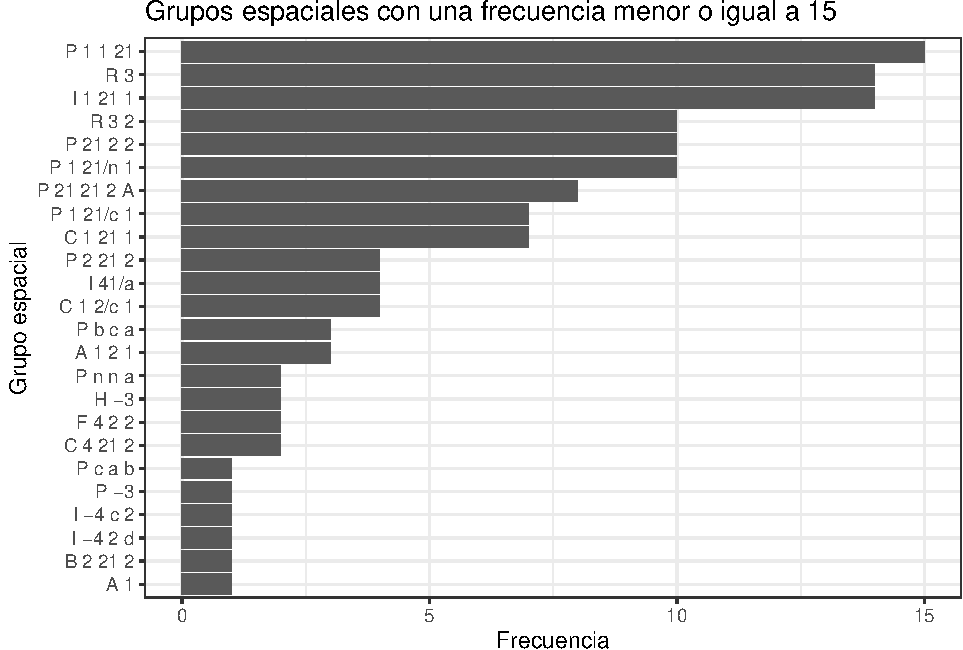
\includegraphics{arrozconleche_files/figure-latex/unnamed-chunk-14-5.pdf}

\begin{Shaded}
\begin{Highlighting}[]
\KeywordTok{ggsave}\NormalTok{(}\StringTok{"histograma\_todo\_xrays\_gpo\_rar.png"}\NormalTok{, }\DataTypeTok{width =} \DecValTok{20}\NormalTok{, }\DataTypeTok{units =} \StringTok{"cm"}\NormalTok{)}
\KeywordTok{ggsave}\NormalTok{(}\StringTok{"histograma\_todo\_xrays\_gpo\_rar.svg"}\NormalTok{, }\DataTypeTok{width =} \DecValTok{20}\NormalTok{, }\DataTypeTok{units =} \StringTok{"cm"}\NormalTok{)}
\CommentTok{\# Genera tablas.}
\CommentTok{\# Tabla de grupos espaciales en el PDB.}
\KeywordTok{kable}\NormalTok{(tab\_gpo) }\OperatorTok{\%\textgreater{}\%}
\StringTok{  }\KeywordTok{kable\_styling}\NormalTok{(}\DataTypeTok{bootstrap\_options =} \KeywordTok{c}\NormalTok{(}\StringTok{"striped"}\NormalTok{, }\StringTok{"hover"}\NormalTok{, }\StringTok{"condensed"}\NormalTok{, }\StringTok{"responsive"}\NormalTok{), }\DataTypeTok{full\_width=}\NormalTok{F)}
\end{Highlighting}
\end{Shaded}

\begin{table}[H]
\centering
\begin{tabular}{l|r}
\hline
gpo & cta\_gpo\\
\hline
P 21 21 21 & 58991\\
\hline
P 1 21 1 & 41319\\
\hline
C 1 2 1 & 21728\\
\hline
C 2 2 21 & 12444\\
\hline
P 21 21 2 & 9650\\
\hline
P 41 21 2 & 8402\\
\hline
P 1 & 8131\\
\hline
P 43 21 2 & 6961\\
\hline
P 31 2 1 & 5712\\
\hline
P 32 2 1 & 5522\\
\hline
I 2 2 2 & 4826\\
\hline
P 61 2 2 & 3139\\
\hline
P 65 2 2 & 2977\\
\hline
H 3 2 & 2804\\
\hline
H 3 & 2518\\
\hline
P 61 & 2321\\
\hline
P 65 & 2046\\
\hline
I 4 2 2 & 1738\\
\hline
P 63 & 1478\\
\hline
P 41 & 1250\\
\hline
P 2 21 21 & 1191\\
\hline
P 31 & 1171\\
\hline
P 32 & 1155\\
\hline
P 43 & 1128\\
\hline
I 41 2 2 & 1090\\
\hline
P 42 21 2 & 1048\\
\hline
P 63 2 2 & 1017\\
\hline
I 4 & 987\\
\hline
P 21 3 & 949\\
\hline
I 2 3 & 799\\
\hline
P 3 2 1 & 738\\
\hline
P 4 21 2 & 629\\
\hline
P 62 2 2 & 593\\
\hline
P 41 2 2 & 591\\
\hline
I 21 3 & 562\\
\hline
P 64 2 2 & 531\\
\hline
I 1 2 1 & 520\\
\hline
P 43 2 2 & 514\\
\hline
I 41 & 485\\
\hline
I 21 21 21 & 467\\
\hline
P 21 2 21 & 465\\
\hline
C 2 2 2 & 454\\
\hline
P 1 2 1 & 439\\
\hline
P 64 & 400\\
\hline
P 6 & 388\\
\hline
P 62 & 365\\
\hline
F 4 3 2 & 323\\
\hline
P 3 & 316\\
\hline
P 41 3 2 & 293\\
\hline
P 2 2 21 & 276\\
\hline
F 2 2 2 & 272\\
\hline
P 32 1 2 & 233\\
\hline
P 31 1 2 & 214\\
\hline
I 4 3 2 & 183\\
\hline
F 2 3 & 175\\
\hline
P 43 3 2 & 166\\
\hline
P 6 2 2 & 166\\
\hline
P 4 & 158\\
\hline
P 42 & 153\\
\hline
I 41 3 2 & 129\\
\hline
P 42 2 2 & 120\\
\hline
P 2 3 & 116\\
\hline
F 41 3 2 & 102\\
\hline
P 4 3 2 & 92\\
\hline
P 4 2 2 & 76\\
\hline
P 42 3 2 & 69\\
\hline
P -1 & 44\\
\hline
B 1 1 2 & 36\\
\hline
P 3 1 2 & 35\\
\hline
P 2 2 2 & 16\\
\hline
P 1 1 21 & 15\\
\hline
I 1 21 1 & 14\\
\hline
R 3 & 14\\
\hline
P 1 21/n 1 & 10\\
\hline
P 21 2 2 & 10\\
\hline
R 3 2 & 10\\
\hline
P 21 21 2 A & 8\\
\hline
C 1 21 1 & 7\\
\hline
P 1 21/c 1 & 7\\
\hline
C 1 2/c 1 & 4\\
\hline
I 41/a & 4\\
\hline
P 2 21 2 & 4\\
\hline
A 1 2 1 & 3\\
\hline
P b c a & 3\\
\hline
C 4 21 2 & 2\\
\hline
F 4 2 2 & 2\\
\hline
H -3 & 2\\
\hline
P n n a & 2\\
\hline
A 1 & 1\\
\hline
B 2 21 2 & 1\\
\hline
I -4 2 d & 1\\
\hline
I -4 c 2 & 1\\
\hline
P -3 & 1\\
\hline
P c a b & 1\\
\hline
\end{tabular}
\end{table}

\begin{Shaded}
\begin{Highlighting}[]
\CommentTok{\# Tabla del tipo de entidades en el PDB.}
\KeywordTok{kable}\NormalTok{(tab\_tde) }\OperatorTok{\%\textgreater{}\%}
\StringTok{  }\KeywordTok{kable\_styling}\NormalTok{(}\DataTypeTok{bootstrap\_options =} \KeywordTok{c}\NormalTok{(}\StringTok{"striped"}\NormalTok{, }\StringTok{"hover"}\NormalTok{, }\StringTok{"condensed"}\NormalTok{, }\StringTok{"responsive"}\NormalTok{), }\DataTypeTok{full\_width=}\NormalTok{F)}
\end{Highlighting}
\end{Shaded}

\begin{table}[H]
\centering
\begin{tabular}{l|r}
\hline
tde & cta\_tde\\
\hline
polypeptide(L) & 210031\\
\hline
polydeoxyribonucleotide & 10913\\
\hline
polyribonucleotide & 5316\\
\hline
polydeoxyribonucleotide/polyribonucleotide hybrid & 175\\
\hline
polypeptide(D) & 83\\
\hline
peptide nucleic acid & 3\\
\hline
other & 2\\
\hline
\end{tabular}
\end{table}

\begin{Shaded}
\begin{Highlighting}[]
\KeywordTok{rm}\NormalTok{(info, df1, datos)}
\CommentTok{\# Guarda los datos como \textasciigrave{}.csv\textasciigrave{}.}
\KeywordTok{write\_excel\_csv}\NormalTok{(df2, }\StringTok{"/run/media/murphy/lolita/doctorado/extract/df2.csv"}\NormalTok{)}
\end{Highlighting}
\end{Shaded}

\hypertarget{limpieza-de-datos}{%
\chapter{Limpieza de datos}\label{limpieza-de-datos}}

Habiendo verificado la integridad de nuestros datos, sigue el turno de su limpieza que consiste en aplicar los siguientes filtros:

\begin{enumerate}
\def\labelenumi{\arabic{enumi}.}
\setcounter{enumi}{-1}
\tightlist
\item
  Elimina entradas donde no se tenga un identificador.
\item
  Elimina entradas con una resolución peor que 2 Å.
\item
  Elimina entradas donde no se anotó el pH en su respectiva columna. Según la \href{http://mmcif.wwpdb.org/dictionaries/mmcif_pdbx_v50.dic/Categories/exptl_crystal_grow.html}{página} del diccionario \texttt{.mmcif} dicha anotación se encuentra en 83.7 \% del total de entradas depositadas en el PDB.
\item
  Elimina entradas donde el número de entidades sea mayor o igual a dos.
\item
  Elimina entradas donde su secuencia de aminoácidos sea muy diferente de la secuencia consenso.
\end{enumerate}

\begin{quote}
Advertencia: Dependiendo de la proteína, la secuencia consenso puede ser igual a la secuencia de la proteína madura en su estado natural o no.
\end{quote}

\begin{enumerate}
\def\labelenumi{\arabic{enumi}.}
\setcounter{enumi}{4}
\tightlist
\item
  Elimina proteínas que no hayan cristalizado en un rango de pH amplio.
\end{enumerate}

\hypertarget{filtros-0-1-y-2}{%
\section{Filtros 0 1 y 2}\label{filtros-0-1-y-2}}

\begin{Shaded}
\begin{Highlighting}[]
\FunctionTok{rm}\NormalTok{ {-}rf /run/media/murphy/lolita/doctorado/clean}
\FunctionTok{mkdir}\NormalTok{ /run/media/murphy/lolita/doctorado/clean}
\end{Highlighting}
\end{Shaded}

\begin{Shaded}
\begin{Highlighting}[]
\CommentTok{\# Filtro 0}
\NormalTok{fil0 \textless{}{-}df2 }\OperatorTok{\%\textgreater{}\%}
\StringTok{  }\KeywordTok{filter}\NormalTok{(}\OperatorTok{!}\NormalTok{ide }\OperatorTok{==}\StringTok{""}\NormalTok{) }\CommentTok{\# Si no tiene identificador se va.}
\CommentTok{\# Filtro 1}
\NormalTok{fil1 \textless{}{-}}\StringTok{ }\NormalTok{fil0 }\OperatorTok{\%\textgreater{}\%}
\StringTok{  }\KeywordTok{filter}\NormalTok{(rs1 }\OperatorTok{\textless{}=}\StringTok{ }\FloatTok{2.0}\NormalTok{) }\CommentTok{\# Mala resolución no me sirve.}
\CommentTok{\# Filtro 2}
\NormalTok{fil2 \textless{}{-}fil1 }\OperatorTok{\%\textgreater{}\%}
\StringTok{  }\KeywordTok{filter}\NormalTok{(}\OperatorTok{!}\KeywordTok{is.na}\NormalTok{(peh)) }\CommentTok{\# Si no tiene pH se va.}
\KeywordTok{setwd}\NormalTok{(}\StringTok{"/run/media/murphy/lolita/doctorado/clean"}\NormalTok{)}
\KeywordTok{write\_excel\_csv}\NormalTok{(fil0, }\StringTok{"fil0.csv"}\NormalTok{)}
\KeywordTok{write\_excel\_csv}\NormalTok{(fil1, }\StringTok{"fil1.csv"}\NormalTok{)}
\KeywordTok{write\_excel\_csv}\NormalTok{(fil2, }\StringTok{"fil2.csv"}\NormalTok{)}
\end{Highlighting}
\end{Shaded}

\hypertarget{filtro-3}{%
\section{Filtro 3}\label{filtro-3}}

\begin{Shaded}
\begin{Highlighting}[]
\BuiltInTok{cd}\NormalTok{ /run/media/murphy/lolita/doctorado/clean}
\FunctionTok{awk}\NormalTok{ {-}F }\StringTok{","} \StringTok{\textquotesingle{}\{print $1\}\textquotesingle{}}\NormalTok{ fil2.csv }\KeywordTok{|} \FunctionTok{tail}\NormalTok{ {-}n +2 }\KeywordTok{|} \FunctionTok{uniq}\NormalTok{ {-}c }\KeywordTok{|} \FunctionTok{sort}\NormalTok{ {-}n }\OperatorTok{\textgreater{}}\NormalTok{ number\_of\_identities\_pdb}
\CommentTok{\# wc {-}l number\_of\_identities\_pdb }
\CommentTok{\# 58961}
\FunctionTok{awk} \StringTok{\textquotesingle{}\{if($1\textgreater{}=2) print $2;\}\textquotesingle{}}\NormalTok{ number\_of\_identities\_pdb }\OperatorTok{\textgreater{}}\NormalTok{ pattern}
\FunctionTok{grep}\NormalTok{ {-}v {-}f pattern fil2.csv }\OperatorTok{\textgreater{}}\NormalTok{ fil3.csv}
\CommentTok{\# wc {-}l fil3.csv }
\CommentTok{\# 50128 fil3.csv}
\end{Highlighting}
\end{Shaded}

\begin{Shaded}
\begin{Highlighting}[]
\CommentTok{\# Carga fil3.}
\NormalTok{fil3 \textless{}{-}}\StringTok{ }\KeywordTok{read\_csv}\NormalTok{(}\StringTok{"/run/media/murphy/lolita/doctorado/clean/fil3.csv"}\NormalTok{)}
\end{Highlighting}
\end{Shaded}

\hypertarget{filtro-4}{%
\section{Filtro 4}\label{filtro-4}}

Saca el identificador, de acuerdo al \emph{top} 50.

\hypertarget{top50}{%
\subsection{Top50}\label{top50}}

Cuenta la frecuencia del identificador de UniProt, con base en esto realiza una lista ordenada en orden descendente.

\begin{quote}
Nota: Digo identificador de UniProt, porque esta es la base de datos que a la que se hace mayor referencia en los archivos del PDB \url{https://www.rcsb.org/pages/help/advancedsearch/uniProtAccessionNumbers}, pero en general puede ser el identificador de cualquier otra base de datos, incluso el mismo PDB.
\end{quote}

\begin{Shaded}
\begin{Highlighting}[]
\NormalTok{fil3cola \textless{}{-}}\StringTok{ }\NormalTok{fil3 }\OperatorTok{\%\textgreater{}\%}
\StringTok{  }\KeywordTok{count}\NormalTok{(ide, }\DataTypeTok{name=}\StringTok{"cta\_ide"}\NormalTok{) }\OperatorTok{\%\textgreater{}\%}\StringTok{ }\CommentTok{\# Colapsa los datos hacia n}
\StringTok{  }\KeywordTok{arrange}\NormalTok{(}\KeywordTok{desc}\NormalTok{(cta\_ide))}
\NormalTok{fil3nocola \textless{}{-}}\StringTok{ }\NormalTok{fil3 }\OperatorTok{\%\textgreater{}\%}\StringTok{ }\CommentTok{\# Agrega n a los datos}
\StringTok{   }\KeywordTok{add\_count}\NormalTok{(ide, }\DataTypeTok{name=}\StringTok{"cta\_ide"}\NormalTok{) }\OperatorTok{\%\textgreater{}\%}
\StringTok{   }\KeywordTok{arrange}\NormalTok{(}\KeywordTok{desc}\NormalTok{(cta\_ide)) }
\CommentTok{\# Una tabla}
\NormalTok{tab\_fil3cola\textless{}{-}}\KeywordTok{head}\NormalTok{(fil3cola, }\DataTypeTok{n=}\DecValTok{50}\NormalTok{) }\CommentTok{\#Aquí escoge n.}
\KeywordTok{kable}\NormalTok{(tab\_fil3cola) }\OperatorTok{\%\textgreater{}\%}
\StringTok{  }\KeywordTok{kable\_styling}\NormalTok{(}\DataTypeTok{bootstrap\_options =} \KeywordTok{c}\NormalTok{(}\StringTok{"striped"}\NormalTok{, }\StringTok{"hover"}\NormalTok{, }\StringTok{"condensed"}\NormalTok{, }\StringTok{"responsive"}\NormalTok{), }\DataTypeTok{full\_width=}\NormalTok{F)}
\end{Highlighting}
\end{Shaded}

\begin{table}[H]
\centering
\begin{tabular}{l|r}
\hline
ide & cta\_ide\\
\hline
P11838 & 689\\
\hline
P00918 & 619\\
\hline
P00698 & 498\\
\hline
P00760 & 310\\
\hline
Q6PJP8 & 296\\
\hline
Q6B0I6 & 269\\
\hline
P02766 & 258\\
\hline
O95696 & 257\\
\hline
Q9UIF8 & 227\\
\hline
P00644 & 216\\
\hline
P00720 & 215\\
\hline
P24941 & 203\\
\hline
P42212 & 182\\
\hline
P29476 & 178\\
\hline
P02185 & 172\\
\hline
O60885 & 170\\
\hline
P18031 & 152\\
\hline
P61823 & 145\\
\hline
P28720 & 144\\
\hline
P07900 & 142\\
\hline
P61626 & 139\\
\hline
P15121 & 125\\
\hline
P56817 & 124\\
\hline
P0DTD1 & 123\\
\hline
P19491 & 116\\
\hline
P23497 & 106\\
\hline
P00800 & 103\\
\hline
O26232 & 102\\
\hline
P22629 & 97\\
\hline
P00489 & 96\\
\hline
P03367 & 96\\
\hline
P68400 & 95\\
\hline
A0A073FPA6 & 84\\
\hline
P46881 & 79\\
\hline
P00811 & 78\\
\hline
Q16539 & 77\\
\hline
P14174 & 75\\
\hline
P00431 & 73\\
\hline
P01116 & 73\\
\hline
P00183 & 72\\
\hline
P01112 & 72\\
\hline
Q00511 & 70\\
\hline
Q76353 & 68\\
\hline
P00282 & 64\\
\hline
P02883 & 63\\
\hline
P02945 & 63\\
\hline
P06873 & 63\\
\hline
P16113 & 63\\
\hline
Q04609 & 63\\
\hline
P00772 & 61\\
\hline
\end{tabular}
\end{table}

\begin{Shaded}
\begin{Highlighting}[]
\KeywordTok{setwd}\NormalTok{(}\StringTok{"/run/media/murphy/lolita/doctorado/clean"}\NormalTok{)}
\KeywordTok{write\_excel\_csv}\NormalTok{(fil3cola, }\StringTok{"fil3cola.csv"}\NormalTok{)}
\KeywordTok{write\_excel\_csv}\NormalTok{(fil3nocola, }\StringTok{"fil3nocola.csv"}\NormalTok{)}
\KeywordTok{write\_excel\_csv}\NormalTok{(tab\_fil3cola, }\StringTok{"tab\_fil3cola.csv"}\NormalTok{)}
\end{Highlighting}
\end{Shaded}

\hypertarget{setup-para-alineamiento-muxfaltiple}{%
\subsection{Setup para alineamiento múltiple}\label{setup-para-alineamiento-muxfaltiple}}

\begin{Shaded}
\begin{Highlighting}[]
\CommentTok{\# Genera el directorio para el alineamiento múltiple.}
\CommentTok{\# Copia las secuencias originales.}
\FunctionTok{rm}\NormalTok{ {-}rf /run/media/murphy/lolita/doctorado/clean/fil4}
\BuiltInTok{cd}\NormalTok{ /run/media/murphy/lolita/doctorado/clean}
\FunctionTok{mkdir}\NormalTok{ {-}p fil4/msa}
\FunctionTok{cp}\NormalTok{ {-}r /home/murphy/ori\_seq /run/media/murphy/lolita/doctorado/clean/fil4/}
\end{Highlighting}
\end{Shaded}

\begin{Shaded}
\begin{Highlighting}[]
\CommentTok{\# Extrae el identificador de las 50 proteínas más representadas en el PDB.}
\NormalTok{ide\_in\_tf3c \textless{}{-}}\StringTok{ }\NormalTok{tab\_fil3cola}\OperatorTok{$}\NormalTok{ide}
\ControlFlowTok{for}\NormalTok{ (j }\ControlFlowTok{in} \KeywordTok{seq}\NormalTok{(}\DecValTok{1}\NormalTok{,}\DecValTok{50}\NormalTok{))}
\NormalTok{\{}
\NormalTok{ide\_i\_ \textless{}{-}ide\_in\_tf3c[[j]]}
\NormalTok{filename \textless{}{-}}\StringTok{ }\KeywordTok{paste}\NormalTok{(}\StringTok{"/run/media/murphy/lolita/doctorado/clean/fil4/msa/"}\NormalTok{, ide\_i\_, }\DataTypeTok{sep=}\StringTok{""}\NormalTok{) }
\CommentTok{\# Escribe un archivo por cada identificador, a partir de fil3.}
\KeywordTok{write\_excel\_csv}\NormalTok{(}\KeywordTok{filter}\NormalTok{(fil3, ide}\OperatorTok{==}\NormalTok{ide\_i\_), filename)}
\NormalTok{\}}
\end{Highlighting}
\end{Shaded}

\hypertarget{consenso}{%
\subsection{Consenso}\label{consenso}}

Crea un alineamiento múltiple de la secuencia canónica de aminoácidos en las estructuras restantes y obtiene una secuencia consenso. Con base en la secuencia consenso, se eliminan entradas del mismo identificador que no sean la misma proteína (sucede cuando el identificador corresponde al gen de una poliproteína, caso de los virus).

\begin{Shaded}
\begin{Highlighting}[]
\BuiltInTok{cd}\NormalTok{ /run/media/murphy/lolita/doctorado/clean/fil4/msa }
\KeywordTok{for} \ExtensionTok{k}\NormalTok{ in }\KeywordTok{\textasciigrave{}}\FunctionTok{ls}\NormalTok{ {-}1rt}\KeywordTok{\textasciigrave{}} \CommentTok{\# Ordenados}
\KeywordTok{do}
\FunctionTok{awk}\NormalTok{ {-}F }\StringTok{","} \StringTok{\textquotesingle{}\{print $1\}\textquotesingle{}} \StringTok{"}\VariableTok{$k}\StringTok{"} \KeywordTok{|} \FunctionTok{tail}\NormalTok{ {-}n +2 }\KeywordTok{|} \FunctionTok{tr} \StringTok{\textquotesingle{}[:upper:]\textquotesingle{}} \StringTok{\textquotesingle{}[:lower:]\textquotesingle{}} \OperatorTok{\textgreater{}}\NormalTok{ pdbs\_}\StringTok{"}\VariableTok{$k}\StringTok{"}
\FunctionTok{sed} \StringTok{\textquotesingle{}s/$/.cif.gz/\textquotesingle{}}\NormalTok{g pdbs\_}\StringTok{"}\VariableTok{$k}\StringTok{"} \OperatorTok{\textgreater{}}\NormalTok{ list\_pdbs\_id\_}\StringTok{"}\VariableTok{$k}\StringTok{"}
\FunctionTok{mkdir}\NormalTok{ sub\_}\StringTok{"}\VariableTok{$k}\StringTok{"}
\FunctionTok{cat}\NormalTok{ list\_pdbs\_id\_}\StringTok{"}\VariableTok{$k}\StringTok{"} \KeywordTok{|} \KeywordTok{while} \BuiltInTok{read} \VariableTok{line}\NormalTok{; }\KeywordTok{do} \FunctionTok{cp}\NormalTok{ /run/media/murphy/lolita/doctorado/PDB\_backup/}\VariableTok{$line}\NormalTok{ /run/media/murphy/lolita/doctorado/clean/fil4/msa/sub\_}\StringTok{"}\VariableTok{$k}\StringTok{"} \KeywordTok{;} \KeywordTok{done} 
\ExtensionTok{/home/murphy/Repos/gemmi/gemmi}\NormalTok{ grep {-}{-}delimiter=}\StringTok{\textquotesingle{}¿\textquotesingle{}}\NormalTok{ \_entity\_poly.entity\_id {-}a \_entity\_poly.type {-}a \_entity\_poly.pdbx\_seq\_one\_letter\_code\_can sub\_}\StringTok{"}\VariableTok{$k}\StringTok{"}\NormalTok{/  }\OperatorTok{\textgreater{}}\NormalTok{ can\_seq\_}\StringTok{"}\VariableTok{$k}\StringTok{"}\NormalTok{.csv}
\FunctionTok{awk}\NormalTok{ {-}F }\StringTok{"¿"} \StringTok{\textquotesingle{}\{print "\textgreater{}"$1"\textbackslash{}n"$4\}\textquotesingle{}}\NormalTok{ can\_seq\_}\StringTok{"}\VariableTok{$k}\StringTok{"}\NormalTok{.csv }\KeywordTok{|} \FunctionTok{sed} \StringTok{\textquotesingle{}s/\textbackslash{}\textbackslash{}n//g\textquotesingle{}} \OperatorTok{\textgreater{}}\NormalTok{ seqs\_}\StringTok{"}\VariableTok{$k}\StringTok{"}\NormalTok{.fa}
\CommentTok{\# Usa mafft para el alineamiento.}
\ExtensionTok{mafft}\NormalTok{ {-}{-}anysymbol {-}{-}quiet {-}{-}op 15 {-}{-}ep 15 {-}{-}addfragments seqs\_}\StringTok{"}\VariableTok{$k}\StringTok{"}\NormalTok{.fa /run/media/murphy/lolita/doctorado/clean/fil4/ori\_seq/ori\_}\StringTok{"}\VariableTok{$k}\StringTok{"}\NormalTok{.fa }\OperatorTok{\textgreater{}}\NormalTok{ msa\_}\StringTok{"}\VariableTok{$k}\StringTok{"}\NormalTok{.afa}
\CommentTok{\# Obtiene la secuencia consenso con cons de EMBOSS.}
\ExtensionTok{cons}\NormalTok{ msa\_}\StringTok{"}\VariableTok{$k}\StringTok{"}\NormalTok{.afa {-}outseq cons\_}\StringTok{"}\VariableTok{$k}\StringTok{"}\NormalTok{ {-}identity 1 {-}datafile EBLOSUM62 {-}sprotein1}
\CommentTok{\# Se verifica visualmente la secuencia consenso en Ugene.}
\FunctionTok{grep}\NormalTok{ {-}v EMBOSS cons\_}\StringTok{"}\VariableTok{$k}\StringTok{"} \KeywordTok{|} \FunctionTok{sed} \StringTok{\textquotesingle{}s/x//g\textquotesingle{}} \KeywordTok{|} \FunctionTok{tr} \StringTok{\textquotesingle{}\textbackslash{}n\textquotesingle{}} \StringTok{\textquotesingle{} \textquotesingle{}} \KeywordTok{|} \FunctionTok{sed} \StringTok{\textquotesingle{}s/ //g\textquotesingle{}} \OperatorTok{\textgreater{}}\NormalTok{ cons\_}\StringTok{"}\VariableTok{$k}\StringTok{"}\NormalTok{\_c}
\KeywordTok{done}
\end{Highlighting}
\end{Shaded}

\begin{verbatim}
## Create a consensus sequence from a multiple alignment
## Create a consensus sequence from a multiple alignment
## Create a consensus sequence from a multiple alignment
## Create a consensus sequence from a multiple alignment
## Create a consensus sequence from a multiple alignment
## Create a consensus sequence from a multiple alignment
## Create a consensus sequence from a multiple alignment
## Create a consensus sequence from a multiple alignment
## Create a consensus sequence from a multiple alignment
## Create a consensus sequence from a multiple alignment
## Create a consensus sequence from a multiple alignment
## Create a consensus sequence from a multiple alignment
## Create a consensus sequence from a multiple alignment
## Create a consensus sequence from a multiple alignment
## Create a consensus sequence from a multiple alignment
## Create a consensus sequence from a multiple alignment
## Create a consensus sequence from a multiple alignment
## Create a consensus sequence from a multiple alignment
## Create a consensus sequence from a multiple alignment
## Create a consensus sequence from a multiple alignment
## Create a consensus sequence from a multiple alignment
## Create a consensus sequence from a multiple alignment
## Create a consensus sequence from a multiple alignment
## Create a consensus sequence from a multiple alignment
## Create a consensus sequence from a multiple alignment
## Create a consensus sequence from a multiple alignment
## Create a consensus sequence from a multiple alignment
## Create a consensus sequence from a multiple alignment
## Create a consensus sequence from a multiple alignment
## Create a consensus sequence from a multiple alignment
## Create a consensus sequence from a multiple alignment
## Create a consensus sequence from a multiple alignment
## Create a consensus sequence from a multiple alignment
## Create a consensus sequence from a multiple alignment
## Create a consensus sequence from a multiple alignment
## Create a consensus sequence from a multiple alignment
## Create a consensus sequence from a multiple alignment
## Create a consensus sequence from a multiple alignment
## Create a consensus sequence from a multiple alignment
## Create a consensus sequence from a multiple alignment
## Create a consensus sequence from a multiple alignment
## Create a consensus sequence from a multiple alignment
## Create a consensus sequence from a multiple alignment
## Create a consensus sequence from a multiple alignment
## Create a consensus sequence from a multiple alignment
## Create a consensus sequence from a multiple alignment
## Create a consensus sequence from a multiple alignment
## Create a consensus sequence from a multiple alignment
## Create a consensus sequence from a multiple alignment
## Create a consensus sequence from a multiple alignment
\end{verbatim}

Los siguientes bloques tienen como objetivo eliminar entradas de la misma proteína donde la distancia en caracteres (sean sustituciones, deleciones o inserciones) sea mayor o igual a 15 con respecto a la secuencia consenso. Esto elimina proteínas con el péptido señal (normalmente arriba de 15) y mantiene proteínas con la cola de histidinas (normalmente abajo de 15).

\begin{Shaded}
\begin{Highlighting}[]
\CommentTok{\# Para cada proteína compara su secuencia canónica con su secuencia consenso.}
\CommentTok{\# Se asigna una etiqueta "Wt" o "NotWt" dependiendo del resultado.}
\ControlFlowTok{for}\NormalTok{ (j }\ControlFlowTok{in} \KeywordTok{seq}\NormalTok{(}\DecValTok{1}\NormalTok{,}\DecValTok{50}\NormalTok{))}
\NormalTok{\{}
\NormalTok{  ide \textless{}{-}ide\_in\_tf3c[[j]] }\CommentTok{\# identificador}
\NormalTok{  file1 \textless{}{-}}\StringTok{ }\KeywordTok{paste}\NormalTok{(}\StringTok{"/run/media/murphy/lolita/doctorado/clean/fil4/msa/can\_seq\_"}\NormalTok{, ide, }\StringTok{".csv"}\NormalTok{, }\DataTypeTok{sep=}\StringTok{""}\NormalTok{)}
\NormalTok{  impo1 \textless{}{-}}\StringTok{ }\KeywordTok{read\_delim}\NormalTok{(file1, }\StringTok{"¿"}\NormalTok{, }\DataTypeTok{escape\_double =} \OtherTok{FALSE}\NormalTok{, }\DataTypeTok{col\_names =} \OtherTok{FALSE}\NormalTok{, }
    \DataTypeTok{comment =} \StringTok{"*\textgreater{}"}\NormalTok{, }\DataTypeTok{trim\_ws =} \OtherTok{TRUE}\NormalTok{)}
\NormalTok{  pdb\textless{}{-}impo1}\OperatorTok{$}\NormalTok{X1}
\NormalTok{  nde\textless{}{-}stringr}\OperatorTok{::}\KeywordTok{str\_replace}\NormalTok{(impo1}\OperatorTok{$}\NormalTok{X2, }\StringTok{\textquotesingle{}�\textquotesingle{}}\NormalTok{, }\StringTok{\textquotesingle{}\textquotesingle{}}\NormalTok{)}
\NormalTok{  tde\textless{}{-}stringr}\OperatorTok{::}\KeywordTok{str\_replace}\NormalTok{(impo1}\OperatorTok{$}\NormalTok{X3, }\StringTok{\textquotesingle{}�\textquotesingle{}}\NormalTok{, }\StringTok{\textquotesingle{}\textquotesingle{}}\NormalTok{)}
\NormalTok{  sec0\textless{}{-}stringr}\OperatorTok{::}\KeywordTok{str\_replace}\NormalTok{(impo1}\OperatorTok{$}\NormalTok{X4, }\StringTok{\textquotesingle{}�\textquotesingle{}}\NormalTok{, }\StringTok{\textquotesingle{}\textquotesingle{}}\NormalTok{)}
\NormalTok{  sec\textless{}{-}stringr}\OperatorTok{::}\KeywordTok{str\_replace\_all}\NormalTok{(sec0, }\StringTok{\textquotesingle{}}\CharTok{\textbackslash{}\textbackslash{}\textbackslash{}\textbackslash{}}\StringTok{n\textquotesingle{}}\NormalTok{, }\StringTok{\textquotesingle{}\textquotesingle{}}\NormalTok{)}
\NormalTok{  oname1 =}\StringTok{ }\KeywordTok{paste}\NormalTok{(}\StringTok{"df"}\NormalTok{, }\StringTok{"\_"}\NormalTok{, ide, }\DataTypeTok{sep=}\StringTok{""}\NormalTok{)}
  \KeywordTok{assign}\NormalTok{(oname1, }\KeywordTok{data.frame}\NormalTok{(pdb, nde, tde, sec))}
\NormalTok{  file2 \textless{}{-}}\StringTok{ }\KeywordTok{paste}\NormalTok{(}\StringTok{"/run/media/murphy/lolita/doctorado/clean/fil4/msa/cons\_"}\NormalTok{, ide, }\StringTok{"\_c"}\NormalTok{, }\DataTypeTok{sep=}\StringTok{""}\NormalTok{)}
\NormalTok{  impo2 \textless{}{-}}\StringTok{ }\KeywordTok{read\_csv}\NormalTok{(file2, }\DataTypeTok{col\_names =} \OtherTok{FALSE}\NormalTok{)}
\NormalTok{  oname2 =}\StringTok{ }\KeywordTok{paste}\NormalTok{(}\StringTok{"cons\_"}\NormalTok{, ide, }\DataTypeTok{sep=}\StringTok{""}\NormalTok{)}
  \KeywordTok{assign}\NormalTok{(oname2, impo2}\OperatorTok{$}\NormalTok{X1)}
\NormalTok{  n\textless{}{-}}\KeywordTok{nrow}\NormalTok{(}\KeywordTok{get}\NormalTok{(oname1))}
\NormalTok{  bad\_seq\textless{}{-}}\KeywordTok{c}\NormalTok{() }\CommentTok{\# Vacío}
    \ControlFlowTok{for}\NormalTok{(i }\ControlFlowTok{in} \KeywordTok{seq}\NormalTok{(}\DecValTok{1}\NormalTok{, n)) \{}
\NormalTok{      y \textless{}{-}}\StringTok{ }\KeywordTok{adist}\NormalTok{(}\KeywordTok{get}\NormalTok{(oname1)}\OperatorTok{$}\NormalTok{sec[i], }\KeywordTok{get}\NormalTok{(oname2))  }
      \ControlFlowTok{if}\NormalTok{(y }\OperatorTok{\textgreater{}=}\StringTok{ }\DecValTok{15}\NormalTok{)}
\NormalTok{      \{bad\_seq \textless{}{-}}\StringTok{ }\KeywordTok{c}\NormalTok{(bad\_seq, }\StringTok{"NotWt"}\NormalTok{)\}}
      \ControlFlowTok{else}
\NormalTok{      \{bad\_seq \textless{}{-}}\StringTok{ }\KeywordTok{c}\NormalTok{(bad\_seq, }\StringTok{"Wt"}\NormalTok{)\}}
\NormalTok{    \}}
  \KeywordTok{assign}\NormalTok{(oname1, }\KeywordTok{cbind}\NormalTok{(}\KeywordTok{get}\NormalTok{(oname1), bad\_seq))}
\NormalTok{  file3 \textless{}{-}}\KeywordTok{paste}\NormalTok{(}\StringTok{"/run/media/murphy/lolita/doctorado/clean/fil4/msa/fil4\_"}\NormalTok{, ide, }\DataTypeTok{sep=}\StringTok{""}\NormalTok{)}
  \KeywordTok{write\_excel\_csv}\NormalTok{(}\KeywordTok{get}\NormalTok{(oname1), file3)}
\NormalTok{\}}
\end{Highlighting}
\end{Shaded}

\begin{Shaded}
\begin{Highlighting}[]
\CommentTok{\# Extrae toda la información, solo para las 50 proteínas más representadas.}
\BuiltInTok{cd}\NormalTok{ /run/media/murphy/lolita/doctorado/clean/fil4/msa/}
\CommentTok{\#awk {-}F "," \textquotesingle{}\{ if ($5=="NotWt") print $1\}\textquotesingle{} fil4\_*  | tr \textquotesingle{}\textbackslash{}n\textquotesingle{} \textquotesingle{} \textquotesingle{}  \textgreater{} bad\_pdbs}
\ExtensionTok{/home/murphy/Repos/gemmi/gemmi}\NormalTok{ grep {-}{-}delimiter=}\StringTok{\textquotesingle{}¿\textquotesingle{}}\NormalTok{ \_entity\_poly.entity\_id {-}a \_entity\_poly.type {-}a \_struct\_ref.pdbx\_db\_accession {-}a \_entity.pdbx\_description {-}a \_exptl\_crystal\_grow.method {-}a \_exptl\_crystal\_grow.pH {-}a \_exptl\_crystal\_grow.pdbx\_details {-}a \_reflns.d\_resolution\_high {-}a \_reflns\_shell.d\_res\_high {-}a \_symmetry.space\_group\_name\_H{-}M {-}a \_citation.pdbx\_database\_id\_DOI sub\_*/ }\OperatorTok{\textgreater{}}\NormalTok{ information\_from\_fil3}
\FunctionTok{cat}\NormalTok{ fil4\_* }\OperatorTok{\textgreater{}\textgreater{}}\NormalTok{ fil4\_todos}
\FunctionTok{grep}\NormalTok{ {-}v bad\_seq fil4\_todos }\OperatorTok{\textgreater{}}\NormalTok{ almost\_fil4}
\end{Highlighting}
\end{Shaded}

\begin{Shaded}
\begin{Highlighting}[]
\CommentTok{\# Aplica finalmente el filtro 4 sobre las 50 proteínas más representadas.}
\KeywordTok{setwd}\NormalTok{(}\StringTok{"/run/media/murphy/lolita/doctorado/clean/fil4/msa"}\NormalTok{)}
\NormalTok{info\_fil3 \textless{}{-}}\StringTok{ }\KeywordTok{read\_delim}\NormalTok{(}\StringTok{"information\_from\_fil3"}\NormalTok{, }\StringTok{"¿"}\NormalTok{, }\DataTypeTok{escape\_double =} \OtherTok{FALSE}\NormalTok{, }\DataTypeTok{col\_names =} \OtherTok{FALSE}\NormalTok{, }\DataTypeTok{comment =} \StringTok{"*\textgreater{}"}\NormalTok{, }\DataTypeTok{trim\_ws =} \OtherTok{TRUE}\NormalTok{)}
\end{Highlighting}
\end{Shaded}

\begin{verbatim}
## Parsed with column specification:
## cols(
##   X1 = col_character(),
##   X2 = col_character(),
##   X3 = col_character(),
##   X4 = col_character(),
##   X5 = col_character(),
##   X6 = col_character(),
##   X7 = col_character(),
##   X8 = col_character(),
##   X9 = col_character(),
##   X10 = col_character(),
##   X11 = col_character(),
##   X12 = col_character()
## )
\end{verbatim}

\begin{Shaded}
\begin{Highlighting}[]
\NormalTok{almost\_fil4 \textless{}{-}}\StringTok{ }\KeywordTok{read\_csv}\NormalTok{(}\StringTok{"almost\_fil4"}\NormalTok{, }\DataTypeTok{col\_names =} \OtherTok{FALSE}\NormalTok{)}
\end{Highlighting}
\end{Shaded}

\begin{verbatim}
## Parsed with column specification:
## cols(
##   X1 = col_character(),
##   X2 = col_double(),
##   X3 = col_character(),
##   X4 = col_character(),
##   X5 = col_character()
## )
\end{verbatim}

\begin{Shaded}
\begin{Highlighting}[]
\NormalTok{almost\_fil4\textless{}{-}}\KeywordTok{rename}\NormalTok{(almost\_fil4, }\DataTypeTok{bad=}\NormalTok{X5)}
\NormalTok{allbadseqs \textless{}{-}}\KeywordTok{select}\NormalTok{(almost\_fil4, bad)}
\NormalTok{nearly\_almost\_fil4\textless{}{-}}\KeywordTok{cbind}\NormalTok{(info\_fil3, allbadseqs)}
\NormalTok{pdb\textless{}{-}nearly\_almost\_fil4}\OperatorTok{$}\NormalTok{X1}
\NormalTok{nde\textless{}{-}stringr}\OperatorTok{::}\KeywordTok{str\_replace}\NormalTok{(nearly\_almost\_fil4}\OperatorTok{$}\NormalTok{X2, }\StringTok{\textquotesingle{}�\textquotesingle{}}\NormalTok{, }\StringTok{\textquotesingle{}\textquotesingle{}}\NormalTok{)}
\NormalTok{tde\textless{}{-}stringr}\OperatorTok{::}\KeywordTok{str\_replace}\NormalTok{(nearly\_almost\_fil4}\OperatorTok{$}\NormalTok{X3, }\StringTok{\textquotesingle{}�\textquotesingle{}}\NormalTok{, }\StringTok{\textquotesingle{}\textquotesingle{}}\NormalTok{)}
\NormalTok{ide\textless{}{-}stringr}\OperatorTok{::}\KeywordTok{str\_replace}\NormalTok{(nearly\_almost\_fil4}\OperatorTok{$}\NormalTok{X4, }\StringTok{\textquotesingle{}�\textquotesingle{}}\NormalTok{, }\StringTok{\textquotesingle{}\textquotesingle{}}\NormalTok{)}
\NormalTok{nom\textless{}{-}stringr}\OperatorTok{::}\KeywordTok{str\_replace}\NormalTok{(nearly\_almost\_fil4}\OperatorTok{$}\NormalTok{X5, }\StringTok{\textquotesingle{}�\textquotesingle{}}\NormalTok{, }\StringTok{\textquotesingle{}\textquotesingle{}}\NormalTok{)}
\NormalTok{tec\textless{}{-}stringr}\OperatorTok{::}\KeywordTok{str\_replace}\NormalTok{(nearly\_almost\_fil4}\OperatorTok{$}\NormalTok{X6, }\StringTok{\textquotesingle{}�\textquotesingle{}}\NormalTok{, }\StringTok{\textquotesingle{}\textquotesingle{}}\NormalTok{)}
\NormalTok{peh\textless{}{-}stringr}\OperatorTok{::}\KeywordTok{str\_replace}\NormalTok{(nearly\_almost\_fil4}\OperatorTok{$}\NormalTok{X7, }\StringTok{\textquotesingle{}�\textquotesingle{}}\NormalTok{, }\StringTok{\textquotesingle{}\textquotesingle{}}\NormalTok{)}
\NormalTok{con\textless{}{-}stringr}\OperatorTok{::}\KeywordTok{str\_replace}\NormalTok{(nearly\_almost\_fil4}\OperatorTok{$}\NormalTok{X8, }\StringTok{\textquotesingle{}�\textquotesingle{}}\NormalTok{, }\StringTok{\textquotesingle{}\textquotesingle{}}\NormalTok{)}
\NormalTok{rs1\textless{}{-}stringr}\OperatorTok{::}\KeywordTok{str\_replace}\NormalTok{(nearly\_almost\_fil4}\OperatorTok{$}\NormalTok{X9, }\StringTok{\textquotesingle{}�\textquotesingle{}}\NormalTok{, }\StringTok{\textquotesingle{}\textquotesingle{}}\NormalTok{)}
\NormalTok{rs2\textless{}{-}stringr}\OperatorTok{::}\KeywordTok{str\_replace}\NormalTok{(nearly\_almost\_fil4}\OperatorTok{$}\NormalTok{X10, }\StringTok{\textquotesingle{}�\textquotesingle{}}\NormalTok{, }\StringTok{\textquotesingle{}\textquotesingle{}}\NormalTok{)}
\NormalTok{gpo\textless{}{-}stringr}\OperatorTok{::}\KeywordTok{str\_replace}\NormalTok{(nearly\_almost\_fil4}\OperatorTok{$}\NormalTok{X11, }\StringTok{\textquotesingle{}�\textquotesingle{}}\NormalTok{, }\StringTok{\textquotesingle{}\textquotesingle{}}\NormalTok{)}
\NormalTok{doi\textless{}{-}stringr}\OperatorTok{::}\KeywordTok{str\_replace}\NormalTok{(nearly\_almost\_fil4}\OperatorTok{$}\NormalTok{X12, }\StringTok{\textquotesingle{}�\textquotesingle{}}\NormalTok{, }\StringTok{\textquotesingle{}\textquotesingle{}}\NormalTok{)}
\NormalTok{sil\textless{}{-}nearly\_almost\_fil4}\OperatorTok{$}\NormalTok{bad}
\NormalTok{closest\_to\_fil4\textless{}{-}}\KeywordTok{tibble}\NormalTok{(pdb, nde, tde, ide, nom, tec, peh, con, rs1, rs2, gpo, doi, sil)}
\KeywordTok{rm}\NormalTok{(pdb, nde, tde, ide, nom, tec, peh, con, rs1, rs2, gpo, doi, sil)}
\CommentTok{\# Cuidado con el tipo de las columnas, de nuevo.}
\NormalTok{closest\_to\_fil4}\OperatorTok{$}\NormalTok{nde\textless{}{-}}\KeywordTok{as.numeric}\NormalTok{(}\KeywordTok{as.character}\NormalTok{((closest\_to\_fil4}\OperatorTok{$}\NormalTok{nde)))}
\NormalTok{closest\_to\_fil4}\OperatorTok{$}\NormalTok{peh\textless{}{-}}\KeywordTok{as.numeric}\NormalTok{(}\KeywordTok{as.character}\NormalTok{((closest\_to\_fil4}\OperatorTok{$}\NormalTok{peh)))}
\NormalTok{closest\_to\_fil4}\OperatorTok{$}\NormalTok{rs1\textless{}{-}}\KeywordTok{as.numeric}\NormalTok{(}\KeywordTok{as.character}\NormalTok{((closest\_to\_fil4}\OperatorTok{$}\NormalTok{rs1)))}
\NormalTok{closest\_to\_fil4}\OperatorTok{$}\NormalTok{rs2\textless{}{-}}\KeywordTok{as.numeric}\NormalTok{(}\KeywordTok{as.character}\NormalTok{((closest\_to\_fil4}\OperatorTok{$}\NormalTok{rs2)))}
\NormalTok{fil4\textless{}{-}}\StringTok{ }\NormalTok{closest\_to\_fil4 }\OperatorTok{\%\textgreater{}\%}
\StringTok{  }\KeywordTok{filter}\NormalTok{(sil}\OperatorTok{==}\StringTok{"Wt"}\NormalTok{) }\CommentTok{\# Las secuencias malas son 666. casifil* tienen 7719 obs.}
\CommentTok{\# fil4 tiene 7719{-}666=7053}
\KeywordTok{write\_excel\_csv}\NormalTok{(fil4, }\StringTok{"/run/media/murphy/lolita/doctorado/clean/fil4.csv"}\NormalTok{)}
\end{Highlighting}
\end{Shaded}

\hypertarget{obtiene-nombres-y-organismos}{%
\section{Obtiene nombres y organismos}\label{obtiene-nombres-y-organismos}}

Por simplicidad trabaja con nombres.

\begin{Shaded}
\begin{Highlighting}[]
\BuiltInTok{cd}\NormalTok{ /run/media/murphy/lolita/doctorado/clean/}
\FunctionTok{rm}\NormalTok{ {-}rf top50}
\FunctionTok{mkdir}\NormalTok{ top50}
\BuiltInTok{cd}\NormalTok{ top50}
\CommentTok{\# Obtiene los identificadores}
\FunctionTok{cp}\NormalTok{ ../tab\_fil3cola.csv .}
\FunctionTok{awk}\NormalTok{ {-}F }\StringTok{","} \StringTok{\textquotesingle{}\{print $1\}\textquotesingle{}}\NormalTok{  tab\_fil3cola.csv }\KeywordTok{|} \FunctionTok{tail}\NormalTok{ {-}n +2 }\OperatorTok{\textgreater{}}\NormalTok{ top50\_uac.lst}
\CommentTok{\# Convierte de lista a línea.}
\FunctionTok{tr} \StringTok{\textquotesingle{}\textbackslash{}n\textquotesingle{}} \StringTok{\textquotesingle{} \textquotesingle{}} \OperatorTok{\textless{}}\NormalTok{ top50\_uac.lst }\OperatorTok{\textgreater{}}\NormalTok{ top50\_uac.ln}
\CommentTok{\# Descarga el script en perl.}
\FunctionTok{wget}\NormalTok{ {-}O get\_info.pl https://raw.githubusercontent.com/murpholinox/usefulscripts/master/uniprot\_batch\_retrieval.pl}
\CommentTok{\# Instala requisitos para correr el programa.}
\CommentTok{\# sudo dnf install \textquotesingle{}perl(LWP::UserAgent)\textquotesingle{} }
\CommentTok{\# sudo dnf install perl{-}LWP{-}Protocol{-}https}
\FunctionTok{chmod}\NormalTok{ u+x get\_info.pl}
\CommentTok{\# Corre el programa.}
\FunctionTok{perl}\NormalTok{ ./get\_info.pl top50\_uac.ln }\OperatorTok{\textgreater{}}\NormalTok{ top50\_wholeinfo.txt}
\CommentTok{\# 1 \# Obtiene nombres.}
\FunctionTok{egrep} \StringTok{"\^{}DE   RecN|\^{}DE   SubN"}\NormalTok{ top50\_wholeinfo.txt }\OperatorTok{\textgreater{}}\NormalTok{ top50\_nombres.txt}
\CommentTok{\# Solo nombres.}
\FunctionTok{awk}\NormalTok{ {-}F }\StringTok{"="} \StringTok{\textquotesingle{}\{print $2\}\textquotesingle{}}\NormalTok{ top50\_nombres.txt }\KeywordTok{|} \FunctionTok{sed} \StringTok{\textquotesingle{}s/,//\textquotesingle{}}\NormalTok{g }\KeywordTok{|} \FunctionTok{sed} \StringTok{\textquotesingle{}s/;//g\textquotesingle{}} \OperatorTok{\textgreater{}}\NormalTok{ top50\_nombres\_fx.txt}
\CommentTok{\# 2 \# Obtiene organismos. }
\FunctionTok{egrep} \StringTok{"\^{}OS"}\NormalTok{ top50\_wholeinfo.txt }\OperatorTok{\textgreater{}}\NormalTok{ top50\_org.txt}
\CommentTok{\# Elimina organismos con doble línea OS}
\FunctionTok{grep}\NormalTok{ {-}v }\StringTok{"\^{}OS   (HIV{-}1)"}\NormalTok{  top50\_org.txt }\OperatorTok{\textgreater{}}\NormalTok{ b}
\FunctionTok{grep}\NormalTok{ {-}v }\StringTok{"\^{}OS   10044"}\NormalTok{ b }\OperatorTok{\textgreater{}}\NormalTok{ c}
\FunctionTok{grep}\NormalTok{ {-}v }\StringTok{"\^{}OS   14847"}\NormalTok{  c }\OperatorTok{\textgreater{}}\NormalTok{ d}
\FunctionTok{grep}\NormalTok{ {-}v }\StringTok{"\^{}OS   (Hal"}\NormalTok{ d }\KeywordTok{|} \FunctionTok{sed} \StringTok{\textquotesingle{}s/\^{}OS   //g\textquotesingle{}} \OperatorTok{\textgreater{}}\NormalTok{ top50\_org\_fx.txt }
\CommentTok{\# Pega los nombres de las proteínas con su identificador y organismo.}
\ExtensionTok{paste}\NormalTok{ {-}d, top50\_uac.lst top50\_nombres\_fx.txt top50\_org\_fx.txt }\OperatorTok{\textgreater{}}\NormalTok{ top50\_final.csv}
\FunctionTok{cp}\NormalTok{ top50\_final.csv /home/murphy/Repos/kaomurph/tabs}
\end{Highlighting}
\end{Shaded}

\begin{verbatim}
## --2020-06-27 12:38:04--  https://raw.githubusercontent.com/murpholinox/usefulscripts/master/uniprot_batch_retrieval.pl
## Resolving raw.githubusercontent.com (raw.githubusercontent.com)... 151.101.24.133
## Connecting to raw.githubusercontent.com (raw.githubusercontent.com)|151.101.24.133|:443... connected.
## HTTP request sent, awaiting response... 200 OK
## Length: 1321 (1.3K) [text/plain]
## Saving to: ‘get_info.pl’
## 
##      0K .                                                     100% 2.40M=0.001s
## 
## 2020-06-27 12:38:10 (2.40 MB/s) - ‘get_info.pl’ saved [1321/1321]
\end{verbatim}

En \texttt{top50\_final.csv} van las cincuenta proteínas más representadas en el PDB que cumplen los primeros cuatro filtros.

\hypertarget{gruxe1ficas}{%
\section{Gráficas}\label{gruxe1ficas}}

Grafica el intervalo de pH.

\begin{Shaded}
\begin{Highlighting}[]
\FunctionTok{mkdir}\NormalTok{ /run/media/murphy/lolita/doctorado/clean/fil4/plots\_all}
\FunctionTok{mkdir}\NormalTok{ /run/media/murphy/lolita/doctorado/clean/fil4/plots\_gt10}
\FunctionTok{mkdir}\NormalTok{ /run/media/murphy/lolita/doctorado/clean/fil4/plots\_bue}
\end{Highlighting}
\end{Shaded}

\begin{Shaded}
\begin{Highlighting}[]
\CommentTok{\#setwd("/run/media/murphy/lolita/doctorado/clean/fil4/plots\_all")}
\CommentTok{\# Histogramas con datos de fil4}
\ControlFlowTok{for}\NormalTok{ (j }\ControlFlowTok{in} \KeywordTok{seq}\NormalTok{(}\DecValTok{1}\NormalTok{,}\DecValTok{50}\NormalTok{))}
\NormalTok{\{}
\NormalTok{id \textless{}{-}tab\_fil3cola}\OperatorTok{$}\NormalTok{ide[j]}
\KeywordTok{ggplot}\NormalTok{(}\KeywordTok{filter}\NormalTok{(fil4, ide}\OperatorTok{==}\NormalTok{id), }\KeywordTok{aes}\NormalTok{(}\DataTypeTok{x=}\KeywordTok{factor}\NormalTok{(gpo), }\DataTypeTok{y=}\NormalTok{peh)) }\OperatorTok{+}\StringTok{ }\KeywordTok{geom\_boxplot}\NormalTok{() }\OperatorTok{+}\StringTok{ }\KeywordTok{coord\_flip}\NormalTok{() }\OperatorTok{+}\StringTok{ }\KeywordTok{ylab}\NormalTok{(}\StringTok{"pH"}\NormalTok{) }\OperatorTok{+}\StringTok{ }\KeywordTok{xlab}\NormalTok{(}\StringTok{"Grupo espacial"}\NormalTok{)}
\CommentTok{\#svgplot\textless{}{-}paste("box\_pH\_by\_gpo\_", id, ".svg", sep="" )}
\CommentTok{\#pngplot\textless{}{-}paste("box\_pH\_by\_gpo\_", id, ".png", sep="" )}
\CommentTok{\#ggsave(svgplot, width = 20, units = "cm") }
\CommentTok{\#ggsave(pngplot, width = 20, units = "cm")}
\NormalTok{\}}
\end{Highlighting}
\end{Shaded}

Se realiza un análisis visual de las gráficas anteriores, básicamente si el gráfico de caja indica que tengo una distribución de pH arriba de tres unidades se mantiene, en caso contrario se descarta.

\begin{Shaded}
\begin{Highlighting}[]
\CommentTok{\#setwd("/run/media/murphy/lolita/doctorado/clean/fil4/plots\_bue")}
\NormalTok{buenas\textless{}{-}}\KeywordTok{c}\NormalTok{(}\StringTok{"P00918"}\NormalTok{, }\StringTok{"P00698"}\NormalTok{, }\StringTok{"P00760"}\NormalTok{, }\StringTok{"P02766"}\NormalTok{, }\StringTok{"P00644"}\NormalTok{, }\StringTok{"P42212"}\NormalTok{, }\StringTok{"P02185"}\NormalTok{, }\StringTok{"O60885"}\NormalTok{, }\StringTok{"P61823"}\NormalTok{, }\StringTok{"P28720"}\NormalTok{, }\StringTok{"P07900"}\NormalTok{, }\StringTok{"P0DTD1"}\NormalTok{, }\StringTok{"P19491"}\NormalTok{, }\StringTok{"O26232"}\NormalTok{, }\StringTok{"P22629"}\NormalTok{, }\StringTok{"P03367"}\NormalTok{, }\StringTok{"P68400"}\NormalTok{, }\StringTok{"Q16539"}\NormalTok{, }\StringTok{"P14174"}\NormalTok{, }\StringTok{"P01116"}\NormalTok{, }\StringTok{"P01112"}\NormalTok{, }\StringTok{"P00282"}\NormalTok{, }\StringTok{"P06873"}\NormalTok{, }\StringTok{"P16113"}\NormalTok{, }\StringTok{"P00772"}\NormalTok{)}
\ControlFlowTok{for}\NormalTok{ (k }\ControlFlowTok{in} \KeywordTok{seq}\NormalTok{(}\DecValTok{1}\NormalTok{,}\KeywordTok{length}\NormalTok{(buenas)))}
\NormalTok{\{}
\KeywordTok{ggplot}\NormalTok{(}\KeywordTok{filter}\NormalTok{(fil4, ide}\OperatorTok{==}\NormalTok{buenas[k]), }\KeywordTok{aes}\NormalTok{(}\DataTypeTok{x=}\NormalTok{peh)) }\OperatorTok{+}\StringTok{ }\KeywordTok{geom\_histogram}\NormalTok{(}\DataTypeTok{binwidth =} \FloatTok{0.5}\NormalTok{) }\OperatorTok{+}\StringTok{ }\KeywordTok{facet\_wrap}\NormalTok{( }\OperatorTok{\textasciitilde{}}\StringTok{ }\NormalTok{gpo) }\OperatorTok{+}\StringTok{ }\KeywordTok{xlab}\NormalTok{(}\StringTok{"pH"}\NormalTok{) }\OperatorTok{+}\StringTok{ }\KeywordTok{ylab}\NormalTok{ (}\StringTok{"Número de entradas"}\NormalTok{) }\OperatorTok{+}\StringTok{ }\KeywordTok{coord\_cartesian}\NormalTok{(}\DataTypeTok{ylim =} \KeywordTok{c}\NormalTok{(}\DecValTok{1}\NormalTok{, }\DecValTok{20}\NormalTok{)) }\OperatorTok{+}\StringTok{ }\KeywordTok{geom\_hline}\NormalTok{(}\DataTypeTok{yintercept=}\DecValTok{5}\NormalTok{, }\DataTypeTok{linetype=}\StringTok{"dashed"}\NormalTok{, }\DataTypeTok{color =} \StringTok{"red"}\NormalTok{)}
\CommentTok{\#svgplot\textless{}{-}paste("hist\_pH\_by\_gpo\_", buenas[k], ".svg", sep="" )}
\CommentTok{\#pngplot\textless{}{-}paste("hist\_pH\_by\_gpo\_", buenas[k], ".png", sep="" )}
\CommentTok{\#ggsave(svgplot, width = 20, units = "cm") }
\CommentTok{\#ggsave(pngplot, width = 20, units = "cm")}
\NormalTok{\}}
\end{Highlighting}
\end{Shaded}

Se realiza un análisis visual de las gráficas anteriores, básicamente si el histograma tiene la mayor parte de sus barras arriba de cinco, se queda, en caso contrario se descarta.

\begin{Shaded}
\begin{Highlighting}[]
\NormalTok{finales\textless{}{-}}\KeywordTok{c}\NormalTok{(}\StringTok{"P00918"}\NormalTok{, }\StringTok{"P00698"}\NormalTok{, }\StringTok{"P00760"}\NormalTok{, }\StringTok{"P02766"}\NormalTok{, }\StringTok{"P42212"}\NormalTok{, }\StringTok{"O60885"}\NormalTok{, }\StringTok{"P19491"}\NormalTok{, }\StringTok{"O26232"}\NormalTok{, }\StringTok{"P00772"}\NormalTok{, }\StringTok{"P00644"}\NormalTok{, }\StringTok{"P03367"}\NormalTok{, }\StringTok{"P68400"}\NormalTok{, }\StringTok{"Q16539"}\NormalTok{, }\StringTok{"P14174"}\NormalTok{)}
\end{Highlighting}
\end{Shaded}

\hypertarget{quuxe9-falta}{%
\chapter{Qué falta?}\label{quuxe9-falta}}

Cristalizar las proteínas, difractarlas\ldots{}

Pensar en los análisis:

\begin{enumerate}
\def\labelenumi{\arabic{enumi}.}
\tightlist
\item
  Composición atómica
\item
  Número y tipo de contactos
\item
  Diferencia entre grupos espaciales (P00698 y P00760) cristalizan en buen intervalo en dos grupos espaciales
\item
  Estimar la dosis absorbida con un PDB modelo y datos de flujo del sincrotrón a usar
\end{enumerate}

\includegraphics{/run/media/murphy/lolita/doctorado/clean/fil5/final_bp_1.png}
\includegraphics{/run/media/murphy/lolita/doctorado/clean/fil5/final_bp_2.png}
\includegraphics{/run/media/murphy/lolita/doctorado/clean/fil5/final_bp_3.png}
\includegraphics{/run/media/murphy/lolita/doctorado/clean/fil5/final_bp_4.png}
\includegraphics{/run/media/murphy/lolita/doctorado/clean/fil5/final_bp_5.png}
\includegraphics{/run/media/murphy/lolita/doctorado/clean/fil5/final_hist_1.png}
\includegraphics{/run/media/murphy/lolita/doctorado/clean/fil5/final_hist_2.png}
\includegraphics{/run/media/murphy/lolita/doctorado/clean/fil5/final_hist_3.png}
\includegraphics{/run/media/murphy/lolita/doctorado/clean/fil5/final_hist_4.png}
\includegraphics{/run/media/murphy/lolita/doctorado/clean/fil5/final_hist_5.png}

  \bibliography{book.bib,packages.bib}

\end{document}
